\documentclass[ignorenonframetext,xcolor=x11names]{beamer}

\definecolor{mun}{RGB}{134,38,51}
\definecolor{mun2}{RGB}{99,102,106}
%\definecolor{mun}{cmyk}{0,.3922,.2392,.1686}
\definecolor{code}{RGB}{0, 0, 128}
\definecolor{code}{gray}{0.95}

\mode<presentation>
{
%  \usetheme{boxes}
%  \usetheme{default}
%  \usetheme{Montpellier}
%  \usetheme{Singapore}
%   \usetheme{Rochester}
%  \usecolortheme{crane}
%  \usecolortheme{dolphin}
%  \usecolortheme{lily}
%  \usecolortheme{orchid}
  \usecolortheme{rose}
  \setbeamercovered{transparent}
%  \usefonttheme[onlymath]{serif}
  \setbeamercolor*{structure}{bg=mun,fg=mun}
  \setbeamercolor*{palette primary}{use=structure,fg=white,bg=structure.fg}
  \setbeamercolor*{palette secondary}{use=structure,fg=white,bg=structure.fg}
  \setbeamercolor*{palette tertiary}{use=structure,fg=white,bg=black}
  \setbeamercolor*{palette quaternary}{fg=white,bg=black}
  \setbeamercolor{section in toc}{fg=black,bg=white}
  \setbeamercolor{alerted text}{use=structure,fg=structure.fg!50!black!80!black}
  \setbeamercolor{titlelike}{parent=palette primary,fg=structure.fg!50!black}
  \setbeamercolor{frametitle}{bg=mun,fg=white}
  \setbeamercolor*{titlelike}{parent=palette primary}

  \setbeamercolor{normal text}{fg=black!90}
  \setbeamercolor{math text}{fg=black}
  \setbeamercolor{quote}{bg=gray!20}
  \setbeamercolor{quotation}{bg=gray!20}
  \setbeamerfont{cite}{size=\scriptsize}
  \setbeamerfont{quote}{size=\footnotesize}
  \setbeamerfont{quotation}{size=\footnotesize}
  \setbeamercolor{red text}{fg=red!75!black}
  \setbeamertemplate{bibliography item}[triangle]
  \setbeamertemplate{enumerate item}[square]
  \setbeamertemplate{blocks}[rounded][shadow=true]
  \setbeamertemplate{navigation symbols}{}
  \setbeamertemplate{footline}[frame number]
}
\usepackage{tcolorbox}
\usepackage{amsmath}
\usepackage{physics}
\usepackage{pgf}
\usepackage[english]{babel}
\usepackage[latin1]{inputenc}
\usepackage{times}
\usepackage[T1]{fontenc}
\usepackage{multicol}
\usepackage{multirow}
\usepackage{fancyvrb}
\usepackage{tabularx}
\usepackage{amsmath}
\usepackage{bbm}
\usepackage{alltt}
\usepackage{hyperref}
\hypersetup{
    colorlinks=true,
    linkcolor=blue,
    filecolor=magenta,      
    urlcolor=blue,
}
\usepackage{minted}
\newminted{cypher}{autogobble,bgcolor=code,breakbytoken,frame=single,framesep=3pt}
\newminted{R}{autogobble,bgcolor=code,breakbytoken,frame=single,framesep=3pt}
\newminted{text}{autogobble,bgcolor=code,breakbytoken,frame=single,framesep=3pt}
\newminted{sql}{autogobble,bgcolor=code,breakbytoken,frame=single,framesep=3pt}
\newminted{bash}{autogobble,bgcolor=code,breakbytoken,python3,frame=single,framesep=3pt}
\newminted{xml}{autogobble,bgcolor=code,breakbytoken,python3,frame=single,framesep=3pt}
\newminted{python}{bgcolor=code,breakbytoken,python3,frame=single,framesep=3pt}
\newminted{html}{autogobble,bgcolor=code,breakbytoken,frame=single,framesep=3pt}
\newminted{js}{autogobble,bgcolor=code,breakbytoken,frame=single,framesep=3pt}
\AtBeginEnvironment{minted}{%
  \renewcommand{\fcolorbox}[4][]{#4} \scriptsize}
\AtEndEnvironment{minted}{%
  \normalsize}

%\newcommand{\Pr}{\operatorname{Pr}}
\newcommand{\argmax}{\operatorname*{argmax}}
\newcommand{\argmin}{\operatorname*{argmin}}
\newcommand{\Ident}{\operatorname{I}}

\author % (optional, use only with lots of authors)
{Joerg Evermann}
% - Give the names in the same order as the appear in the paper.
% - Use the \inst{?} command only if the authors have different
%   affiliation.

\institute%[Universities of Somewhere and Elsewhere] % (optional, but mostly needed)
{
  Faculty of Business Administration\\
  Memorial University of Newfoundland \\ 
  \texttt{jevermann@mun.ca} 
}

\date{}

\pgfdeclareimage[width=1.5cm]{university-logo}{../MUN_LOGO_CMYK}
\logo{\pgfuseimage{university-logo}}

% If you wish to uncover everything in a step-wise fashion, uncomment
% the following command: 

%\beamerdefaultoverlayspecification{<+->}


\title{Business 4720 - Class 19}

\subtitle{Interpretable Machine Learning -- Explainable AI}

\begin{document}

\begin{frame}{}
  \titlepage
  \footnotesize
  \begin{center}

\includegraphics[height=.5in]{../by-nc.png}

Unless otherwise indicated, the copyright in this material is owned by Joerg Evermann. This material is licensed to you under the \href{https://creativecommons.org/licenses/by-nc/4.0/}{Creative Commons by-attribution non-commercial license (CC BY-NC 4.0)}
\end{center}

\end{frame}

\section{Introduction}

\begin{frame}{This Class}

\begin{block}{What You Will Learn:}
\begin{itemize}
  \item Introduction to Interpetability and Explainability
  \item Model specific and Model agnostic methods
  \item Global explainability
  \item Local explainability
\end{itemize}
\end{block}
\end{frame}

\begin{frame}{Based On}
\begin{block}{}
Molnar, Christoph: \emph{Interpretable Machine Learning} (2023) \\

\vspace{\baselineskip}
\small
\url{https://christophm.github.io/interpretable-ml-book/} \\

\vspace{\baselineskip}
(CC BY-NC-SA License)
\end{block}

\end{frame}

\begin{frame}{Additional Materials}
\small
\begin{block}{SciKit Learn}
A machine learning framework for Python that also provides some interpretable ML functions.

\url{https://scikit-learn.org/stable/user_guide.html}
\end{block}

\begin{block}{LIME}
A Python package to compute Local Interpretable Model Explanations (a local model-agnostic method).

\url{https://github.com/marcotcr/lime}
\end{block}
\begin{block}{SHAP}
A Python package to compute Shapley Additive Explanations (a local model-agnostic interpretation method).

\url{https://shap.readthedocs.io/en/latest/}
\end{block}
\end{frame}

\begin{frame}[fragile]{Tools}
Install required Python packages:
\begin{bashcode}
pip install statsmodels matplotlib scikit-learn \
    PyALE lime shap
\end{bashcode}
\end{frame}


\begin{frame}{Importance of Interpretability}

\begin{quote} \large
Human understanding of how the AI works and arrives at its results (decisions, predictions, \ldots)
\end{quote}

\footnotesize
\begin{itemize}
\item Curiosity
\item Human learning
\item Human sensemaking of events and phenomena
\item Knowledge extraction for scientific progress
\item Safety and compliance assessment
\item Reliability and robustness evaluation
\item Identify knowledge limits
\item Auditability
\item Bias detection \& ensuring fairness
\item Trust and acceptance
\item Debugging \& failure analysis
\item Legal obligations (''right to explanation'')
\end{itemize}
\end{frame}

\begin{frame}{Model Interpretability}
\begin{block}{Distinctions}
\begin{itemize}
   \item Intrinsic $\leftrightarrow$ Post-hoc
   \item Local $\leftrightarrow$ Global
\end{itemize}
\end{block}
%\begin{block}{Result of interpretation method}
%\begin{itemize}
  %\item Feature summary statistics and visualizations
  %\item Model internals (e.g. learned weights, feature visualization)
  %\item Data points (e.g. counterfactuals, predicted class prototypes)
%\end{itemize}
%\end{block}
\end{frame}

%\begin{frame}{Scope of Interpretability}
%\small
%\begin{itemize}
   %\item Model and design transparency \\
    %\hspace{.25in}\emph{''Why does the model have the specific architecture?''}
   %\item Algorithmic transparency \\
    %\hspace{.25in}\emph{''How does the algorithm create the trained model?''}
   %\item Global, holistic model interpretability \\
    %\hspace{.25in}\emph{''How does the trained model make predictions?''}
   %\item Global, modular model interpretability \\
    %\hspace{.25in}\emph{''How do parts of the model affect predictions?''}
   %\item Local interpretability for a single prediction \\
    %\hspace{.25in}\emph{''Why did the model make this prediction for this instance?''}
   %\item Local interpretability for a group of predictions \\
    %\hspace{.25in}\emph{''Why did the model make these predictions for these instances?''}
%\end{itemize}
%\end{frame}

%\begin{frame}{Evaluating Interpretability}
%\begin{itemize}
   %\item Application level (real task)
   %\item Human level (simple tasks)
   %\item Function level (proxy tasks)
%\end{itemize}
%\end{frame}

%\begin{frame}{Properties of Explanations}
%Good explanations have:
%\begin{itemize}
   %\item Accuracy
   %\item Fidelity
   %\item Consistency (between different models)
   %\item Stability (between different instances)
   %\item Comprehensibility
   %\item Explanation of certainty/confidence
   %\item Explanation of data novelty/closeness
   %\item Representativeness (across different instances)
%\end{itemize}
%\end{frame}

%\begin{frame}{Comprehensible Explanations}
%Humand-understandable explanations are:
%\begin{itemize}
   %\item Contrastive
   %\item Selective
   %\item Audience appropriate
   %\item Focus on the exception
   %\item Truthful
   %\item Consistent with prior beliefs
   %\item General
%\end{itemize}
%\end{frame}

\begin{frame}{Intrinsically Interpretable Models}

\centering
\renewcommand{\arraystretch}{1.1}

\begin{tabular}{lccc} \hline
Algorithm & Linear & Monotone & Interaction \\ \hline
\textbf{Linear regression} & Yes & Yes & No  \\ 
Logistic regression & No & Yes & No  \\
\textbf{Decision trees} & No & Some & Yes  \\
RuleFit & Yes & No & Yes  \\
Naive Bayes & No & Yes & No \\
k-NN & No & No & No  \\ \hline
\end{tabular} \\

\scriptsize Source: \url{https://christophm.github.io/interpretable-ml-book/simple.html}\normalsize
\end{frame}

\begin{frame}[fragile]{Linear Regression}
\begin{Rcode}
# Load the bike rental data set
d <- read.csv('https://evermann.ca/busi4720/bike.csv')
# Perform the regression and summarize results
summary(lm(cnt~season+temp, data=d))
\end{Rcode}
Results:
\begin{textcode}
Coefficients:
             Estimate Std. Error t value Pr(>|t|)    
(Intercept)   3151.02     169.35  18.606  < 2e-16 ***
seasonSPRING  -494.15     163.28  -3.026  0.00256 ** 
seasonSUMMER  -852.68     209.82  -4.064 5.35e-05 ***
seasonWINTER -1342.87     164.59  -8.159 1.49e-15 ***
temp           132.79      11.02  12.046  < 2e-16 ***
---
Residual standard error: 1433 on 726 degrees of freedom
Multiple R-squared: 0.4558, Adjusted R-squared: 0.4528 
\end{textcode}
\end{frame}

\begin{frame}{Linear Regression}
\begin{itemize}
   \item \textbf{Algorithmic transparency}: The ordinary least squares loss function is clear and intuitive; provides optimality guarantees
   \item \textbf{Coefficients $\beta$}
   \begin{itemize}
      \item An increase of one unit of a predictor increases the prediction by $\beta$, \emph{assuming all other predictors remain the same} (''ceteris paribus'')
      \item Switching from the reference category (see ''contrasts'') to another category increases the prediction by $\beta$, \emph{assuming all other predictors remain the same} (''ceteris paribus'')
      \item \textbf{Intercept} is the predicted value when all other predictors are 0. Is this reasonable?
   \end{itemize}
   \item $R^2$ is the amount of explained variance; model weights should only be interpreted when $R^2$ reasonable size.
   \item \textbf{Relative feature importance} is given by the $t=\frac{\hat{\beta}}{SE(\hat{\beta})}$ statistic.
\end{itemize}
\end{frame}

%\begin{frame}{Linear Regression}
%\begin{block}{Effects Plot}
%\begin{align*}
%\operatorname{effect}_j^{(i)} = \beta_j x_j^{(i)}
%\end{align*}
%\centering
%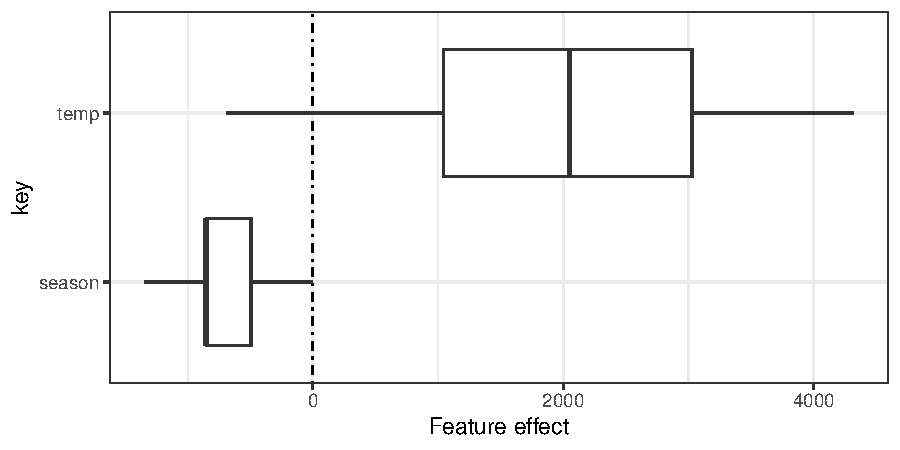
\includegraphics[height=2in]{effect_plot_lm.pdf}
%\end{block}
%\end{frame}

%\begin{frame}[fragile]{Linear Regression}
%\begin{Rcode}
%> bike$cnt[6]
%[1] 1606
%> bike$temp[6]
%[1] 1.604356
%> bike$season[6]
%[1] WINTER
%> coef(fitted)
 %(Intercept) seasonWINTER         temp 
   %3151.0170   -1342.8730     132.7946 
%\end{Rcode}
%\begin{center}
%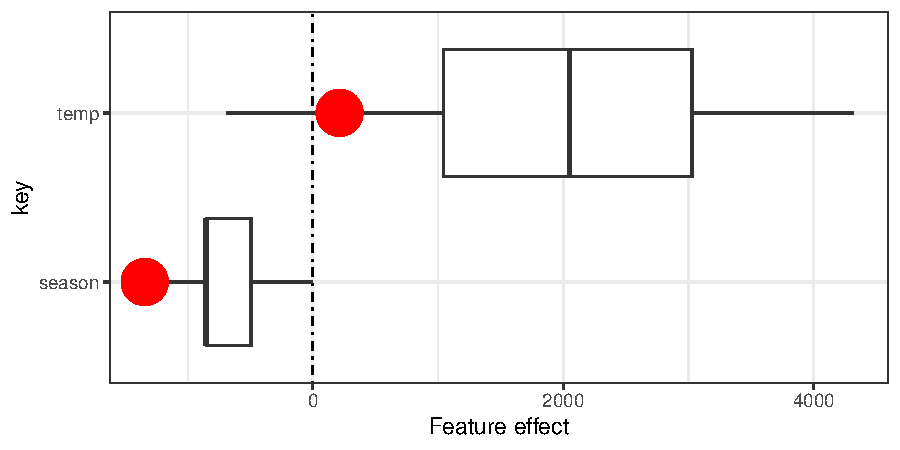
\includegraphics[height=1.5in]{effect_plot_2.pdf}
%\end{center}
%\end{frame}

\begin{frame}[fragile]{Linear Regression}
\textbf{Dimension reduction} to improve interpretability:
\begin{itemize}
   \item Manual feature selection, e.g. based on effect size
   \item Automatic feature selection (forwards or backwards)
   \item Regression with PCA components
   \item Penalized regression with LASSO
\end{itemize} 

Be aware of bias-variance trade-off with all of these. \\

%\textbf{LASSO Example}:
%\begin{Rcode}
%library(glmnet)
%x <- model.matrix(cnt ~ ., bike)[,-1]
%y <- bike$cnt
%cv.out <- cv.glmnet(x, y, type.measure='mse')
%fitted.lasso <- glmnet(x, y, lambda=cv.out$lambda.min)
%\end{Rcode}
\end{frame}


\begin{frame}{Decision Trees}

\begin{block}{Decision Tree Types}
\begin{itemize}
\item Regression trees
\item Classification trees
\end{itemize}
\end{block}

\begin{block}{Strengths}
\begin{itemize}
   \item Intrinsically interpretable and visualizable
   \item Individual predictions explained by path through tree
   \item Captures feature interactions
   \item No need to transform features
\end{itemize}
\end{block}

\begin{block}{Weaknesses}
\begin{itemize}
   \item Unstable (high variance)
   \item Tend to overfit
   \item Predictions are piecewise constant
\end{itemize}
\end{block}

\end{frame}

\begin{frame}{Regression Trees}
\begin{columns}
\begin{column}{.8\textwidth}
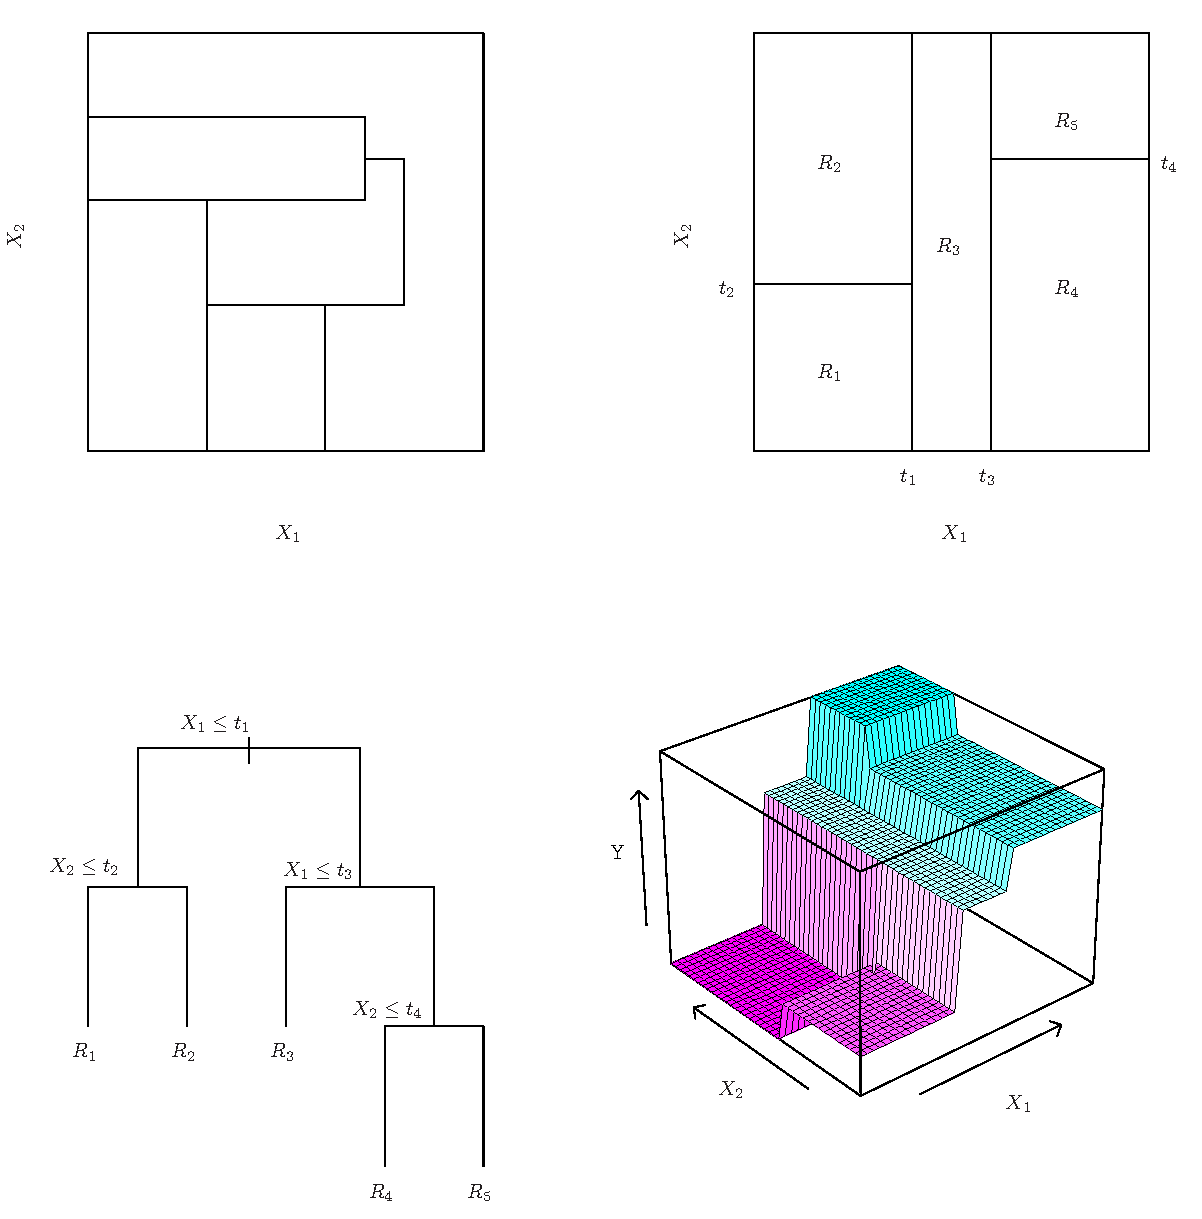
\includegraphics[height=3.25in]{../class11/Figures_Chapters_7-13/Chapter8/8_3.pdf} 
\end{column}
\begin{column}{.2\textwidth}
\scriptsize Source: ISLR2 Figure 8.3
\end{column}
\end{columns}
\end{frame}

\begin{frame}{Regression Trees}
\begin{enumerate}
   \item Recursively divide the predictor space into $J$ distinct and non-overlapping regions $R_1, R_2, \ldots, R_j$
   \begin{itemize}
   \vspace{\baselineskip}
       \item For every predictor $j$ and split point $s$ define regions
       \begin{align*}
       R_1(j,s) = \{X | X_j < s\} \quad &\text{and} \quad R_2(j, s) = \{X | X_j \geq s\}
       \end{align*}
       \item Choose $j$ and $s$ to minimize variance in each region:
       \begin{align*}
       \sum_{i: x_i \in R_1(j,s)} (y_i - \bar{y}_{R_1})^2 &+ \sum_{i: x_i \in R_2(j,s)} (y_i - \bar{y}_{R_2})^2
       \end{align*}
   \end{itemize}
   \item For every observation that falls into region $R_j$, prediction is the mean of the targets of training observations in $R_j$
\end{enumerate}
\end{frame}

\begin{frame}[fragile]{Regression Trees}
Prepare data:
\begin{pythoncode}
import matplotlib.pyplot as plt
import pandas as pd
d=pd.read_csv('https://evermann.ca/busi4720/bike.csv')
x=d[['temp', 'hum']]
y=d['cnt']
\end{pythoncode}
Fit unpruned tree:
\begin{pythoncode}
from sklearn.tree import DecisionTreeRegressor
regr = DecisionTreeRegressor()
regr.fit(x, y)
\end{pythoncode}
Print the MSE:
\begin{pythoncode}
from sklearn.metrics import mean_squared_error
mean_squared_error(regr.predict(x), y)
\end{pythoncode}
\end{frame}

\begin{frame}[fragile]{Regression Trees}
Print the tree:
\begin{pythoncode}
import sklearn
print (sklearn.tree.export_text(regr, \
    feature_names=x.columns))
\end{pythoncode}
Plot the tree:
\begin{pythoncode}
sklearn.tree.plot_tree(regr, 
    max_depth=2, feature_names=x.columns,
    filled=True, fontsize=6)
plt.show()
\end{pythoncode}
Early stopping can prevent overfitting and maintain interpretability:
\begin{pythoncode}
regr = DecisionTreeRegressor(max_depth=3)
regr = DecisionTreeRegressor(min_samples_leaf=10)
regr = DecisionTreeRegressor(max_leaf_nodes=8)
\end{pythoncode}
\end{frame}

\begin{frame}{Regression Trees}
\centering
%\hspace{-.5in}
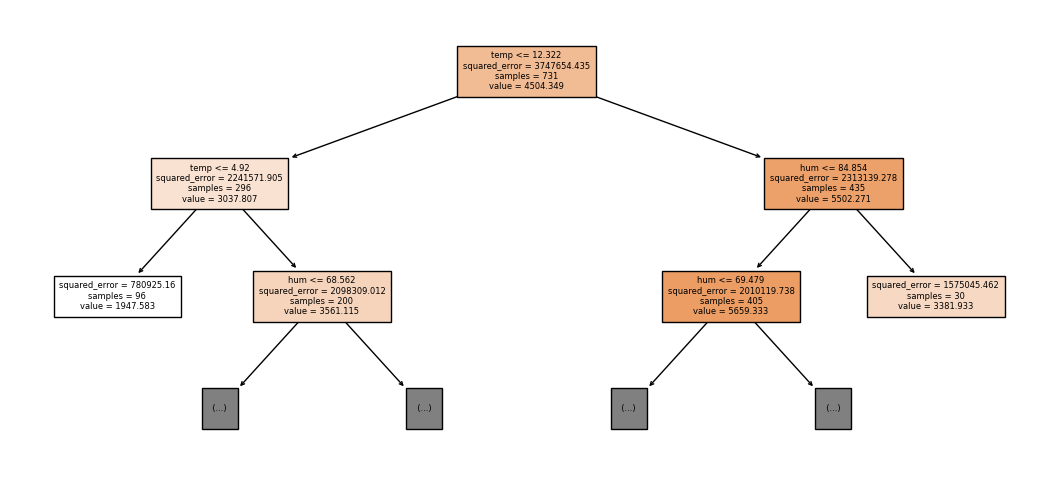
\includegraphics[width=\textwidth]{reg_tree.png}
\end{frame}

\begin{frame}[fragile]{Regression Trees}
Plot fitted versus true values:
\begin{pythoncode}
import plotly.express as px
px.scatter(pd.DataFrame([y, regr.predict(x)], \
    index=['y', 'yhat']).transpose() \
        ,x='y', y='yhat').show()
\end{pythoncode}
\end{frame}

\begin{frame}{Regression Trees}

\centering

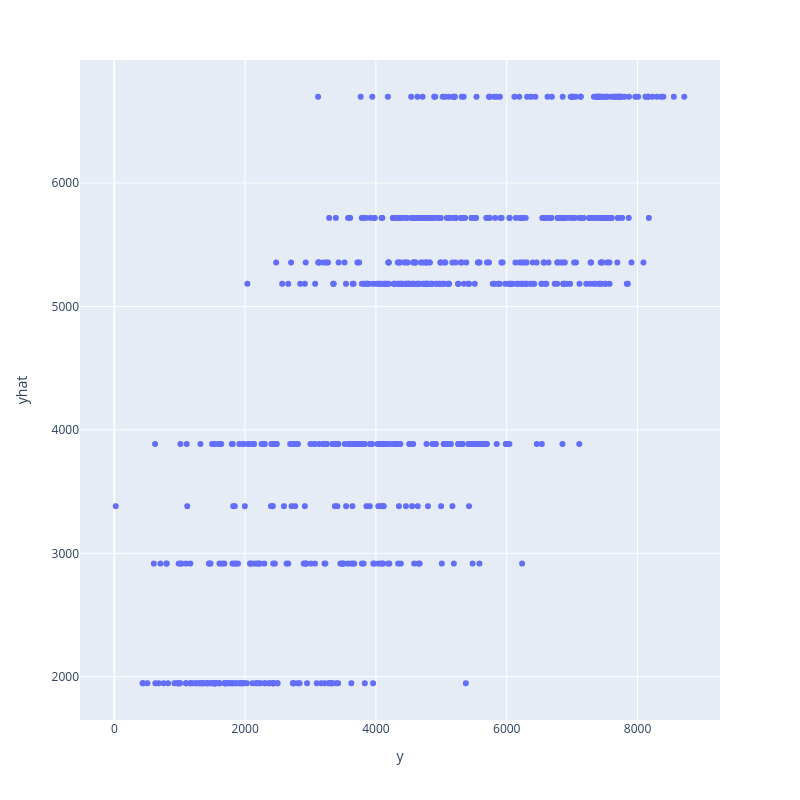
\includegraphics[height=3.25in]{tree_fitted_true.png}
\end{frame}

\begin{frame}{Hands-On Exercises}
Fit regression trees to the bike dataset on the previous slides. Calculate the MSE, print the decision rules, and plot predicted versus true values as you vary:
\begin{itemize}
   \item \textbf{max\_depth}: choose values 1, 3, 5, 7
   \item \textbf{min\_samples\_leaf}: choose values 1, 5, 10, 20
   \item \textbf{max\_leaf\_nodes}: choose values 2, 8, 16, 32
\end{itemize}
How does the training MSE change? What can you observe from the plots of predicted versus true values?
\end{frame}

%\begin{frame}{Regression Trees -- Pruning}
%\textbf{Cost Complexity Pruning}
%\begin{itemize}
%\item Regularization (prevent overfitting)
%\item Improved interpretability
%\item Pruning by ''penalized'' loss function
%\item Penalty for tree complexity, i.e. number of terminal nodes
%\end{itemize}
%\begin{align*}
%\min_\alpha \quad \sum_{m=1}^{|T|} \sum_{i: x_i \in R_m} (y_i - \bar{y}_{R_m})^2 + \alpha |T|
%\end{align*}
%\begin{itemize}
   %\item $|T|$ is the number of terminal nodes of $T$
   %\item $\alpha$ is a tuning parameter, determined by cross-validation
   %\item $m$ counts terminal nodes
%\end{itemize}
%\end{frame}


%\begin{frame}[fragile]{Regression Trees -- Pruning}
%Prune the tree using cost-complexity and cross-validation:
%\begin{pythoncode}
%from sklearn.model_selection import train_test_split
%x_train, x_test, y_train, y_test=train_test_split(x,y)

%# Calculate the alphas and corresponding MSE
%p=regr.cost_complexity_pruning_path(x_train, y_train)
%alphas, mses = p.ccp_alphas, p.impurities

%# Plot
%import matplotlib.pyplot as plt
%fig, ax = plt.subplots()
%ax.plot(alphas,mses,marker="o",drawstyle="steps-post")
%ax.set_xlabel("alpha")
%ax.set_ylabel("MSE")
%ax.set_title("MSE versus alpha")
%\end{pythoncode}
%\end{frame}

%\begin{frame}{Regression Tree -- Pruning}
%MSE versus $\alpha$: \\
%\begin{center}
%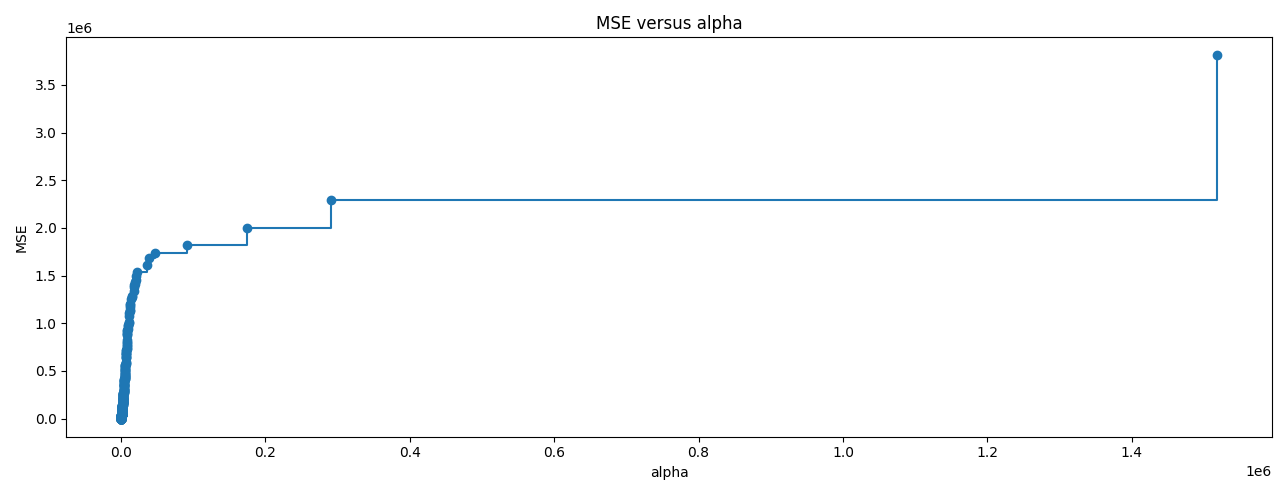
\includegraphics[width=.75\textwidth]{tree_mse_alpha.png}
%\end{center}
%\end{frame}

%\begin{frame}[fragile]{Regression Trees -- Pruning}
%Fit trees for possible alphas:
%\begin{pythoncode}
%regrs = []
%for alpha in alphas:
    %regr = DecisionTreeRegressor(ccp_alpha=alpha)
    %regr.fit(x_train, y_train)
    %regrs.append(regr)
%\end{pythoncode}
%Node count and depth of tree:
%\begin{pythoncode}
%node_counts = [regr.tree_.node_count for regr in regrs]
%depth = [regr.tree_.max_depth for regr in regrs]
%\end{pythoncode}
%\end{frame}

%\begin{frame}{Regression Trees -- Pruning}
%\begin{center}
%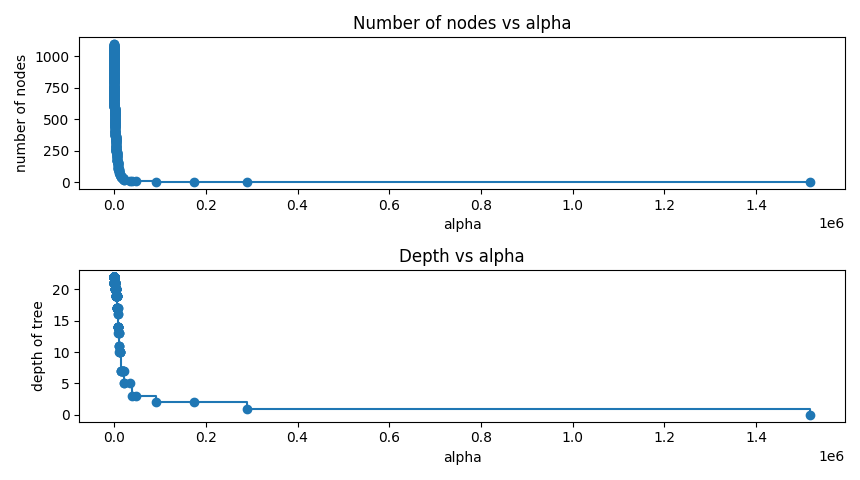
\includegraphics[width=.8\textwidth]{tree_nodes_alpha.png}
%\end{center}
%\end{frame}

%\begin{frame}[fragile]{Regression Trees}
%Compute train and test MSEs for all regression trees:
%\begin{pythoncode}
%train_mses = [sum((regr.predict(x_train)-y_train)**2) \
    %/len(y_train) for regr in regrs]
%test_mses = [sum((regr.predict(x_test)-y_test)**2) \
    %/len(y_train) for regr in regrs]
%min_mse = min(test_mses)
%alpha_opt = alphas[test_mses.index(min(test_mses))]
%\end{pythoncode}
%\begin{center}
%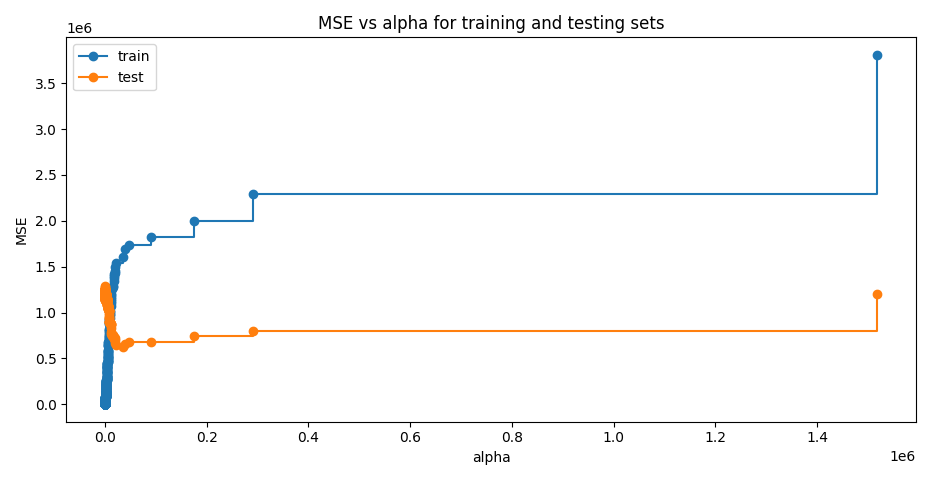
\includegraphics[width=.85\textwidth]{tree_cv_mse_alpha.png}
%\end{center}
%\end{frame}

\begin{frame}{Classification Trees}
\begin{itemize}
   \item Instead of mean, predict most common class in leaf node.
   \item Instead of MSE, use \textbf{Gini index} $G$ (node purity) to determine splits:
   \begin{align*}
   G &= \sum_{k=1}^K \hat{p}_{mk}(1 - \hat{p}_{mk})
   \end{align*} 
   \item Instead of Gini index, use \textbf{Entropy} $H$ as loss functions to determine splits:
   \begin{align*}
   H &= - \sum_{k=1}^K \hat{p}_{mk} \log \hat{p}_{mk} 
   \end{align*}
   \item Tree pruning using classification error rate
\end{itemize}
\end{frame}

\begin{frame}{Decision Trees}
Further reading: \\

\small
\url{https://scikit-learn.org/stable/modules/tree.html} \\

\url{https://scikit-learn.org/stable/auto_examples/tree/plot_unveil_tree_structure.html} \\

\url{https://scikit-learn.org/stable/auto_examples/tree/plot_cost_complexity_pruning.html}
\end{frame}


%\begin{frame}{Model Agnostic Methods}
%\begin{block}{Advantages}
%\begin{itemize}
   %\item Model flexibility
   %\item Explanation flexibility
   %\item Representation flexibility
%\end{itemize}
%\end{block}
%\end{frame}

\begin{frame}{Global Model Agnostic Methods}
\begin{itemize}
    \item \textbf{Partial dependence plot (PDP)}
    \item \textbf{Individual conditional expectation (ICE) curves} 
    \item \textbf{Accumulated local effects plot (ALE)}
    \item Feature interaction
    \item Functional decomposition
    \item \textbf{Permutation feature importance}
    \item \textbf{Global surrogate models}
    \item Prototypes
\end{itemize}
\end{frame}

\begin{frame}[fragile]{Partial Dependence Plot (PDP)}
Marginal effect of one or a few features $X_S$ on the outcome, marginalized (i.e. sum weighted by probability) over all other (complement) features $X_C$.
\begin{align*}
\hat{f}_S(X_S) &= \mathbbm{E}_{X_C} \left[ \hat{f}(X_S, X_C)) \right] = \int \hat{f}(X_S, X_C) p(X_C) dX_c 
\intertext{Estimated from sample data as:}
\hat{f}_S(X_S) &= \frac{1}{n}\sum_{i=1}^n \hat{f}(X_S, X_C^{(i)})
\end{align*}

Shows how the \emph{average} prediction changes when the focal predictor is changed (assuming feature independence). 

\end{frame}

%\begin{frame}[fragile]{Partial Dependence Plot (PDP)}
%A simple linear regression example
%\begin{pythoncode}
%import matplotlib.pyplot as plt
%import pandas as pd
%d=pd.read_csv('https://evermann.ca/busi4720/bike.csv')
%x=pd.get_dummies(d)
%y=x.pop('cnt')

%from sklearn import linear_model
%regr = linear_model.LinearRegression()
%regr.fit(x, y)

%from sklearn.inspection import PartialDependenceDisplay
%PartialDependenceDisplay \
    %.from_estimator(regr, x, [1, 2, (1,2)])
%plt.show()
%\end{pythoncode}
%\end{frame}

%\begin{frame}{Partial Dependence Plot (PDP)}
%\centering

%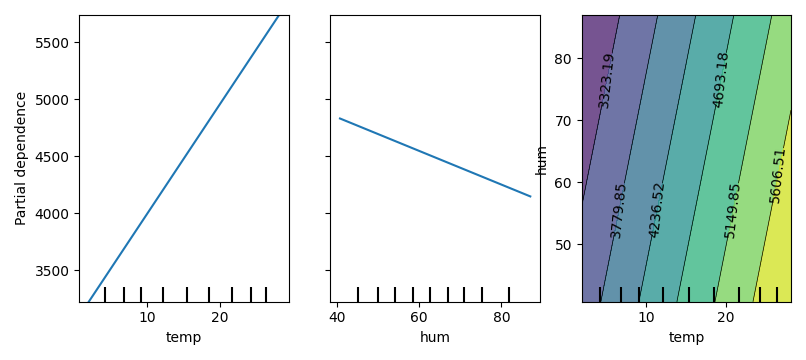
\includegraphics[width=\textwidth]{pdp_lm.png}
%\end{frame}

\begin{frame}[fragile]{Partial Dependence Plot (PDP)}
Read the data set:
\begin{pythoncode}
import pandas as pd
d=pd.read_csv('https://evermann.ca/busi4720/bike.csv')
x=d[['temp', 'hum']]
y=d[['cnt']]
\end{pythoncode}
Fit a regression tree:
\begin{pythoncode}
from sklearn.tree import DecisionTreeRegressor
regr = DecisionTreeRegressor(max_depth=5).fit(x, y)
\end{pythoncode}
Show the PDP:
\begin{pythoncode}
import matplotlib.pyplot as plt
from sklearn.inspection import PartialDependenceDisplay
PartialDependenceDisplay \
    .from_estimator(regr, x, [0, 1, (0,1)],
        grid_resolution=20)
plt.show()
\end{pythoncode}
\end{frame}

\begin{frame}{Partial Dependence Plot (PDP)}
\begin{center}
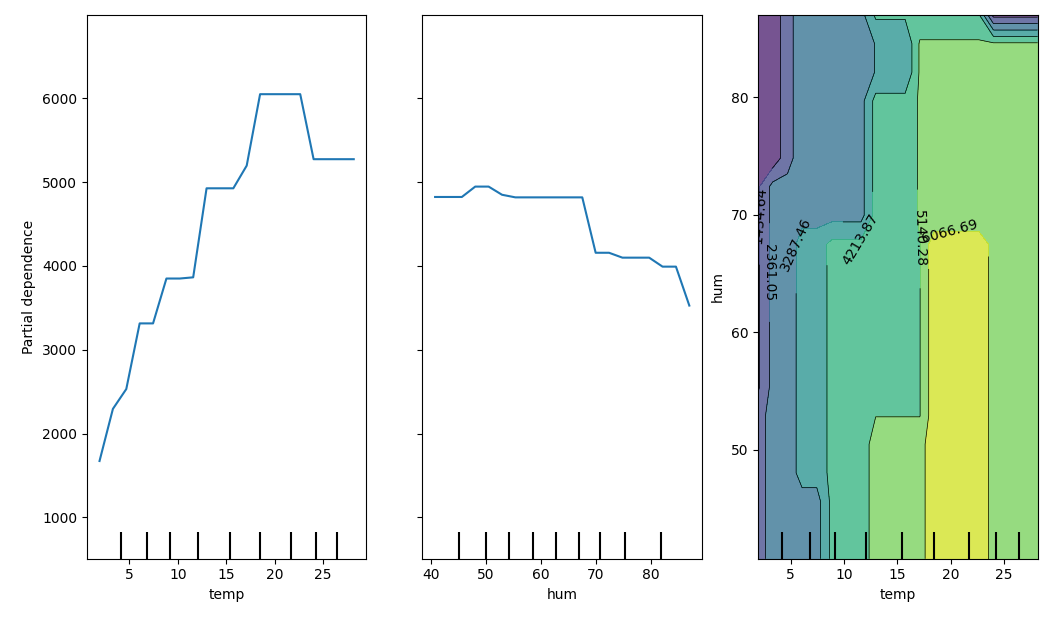
\includegraphics[width=\textwidth]{pdp_dtr.png}
\end{center}
\end{frame}

\begin{frame}[fragile]{Individual Conditional Expectation (ICE) Plot}
\begin{itemize}
\item Instead of the average effect of a feature, shows PDP for individual samples
\item Identify individual \textbf{outlier} cases or \textbf{heterogeneous data}
\end{itemize} 
\begin{pythoncode}
PartialDependenceDisplay \
    .from_estimator(regr, x, [0, 1], kind='both')
\end{pythoncode}
\begin{center}
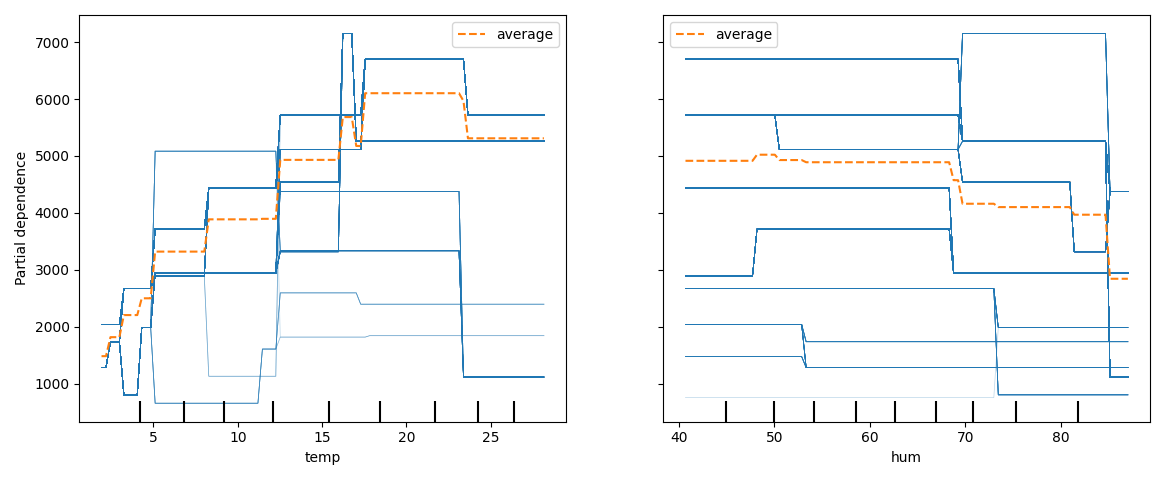
\includegraphics[width=.75\textwidth]{ice_pdp_reg.png}
\end{center}

\footnotesize (Individual samples overlaid due to piece-wise constant regression)
\end{frame}

\begin{frame}[fragile]{Accumulated Local Effects (ALE) Plot}
\begin{itemize}
   \item Effects computed for a grid of intervals (a ''local window'') (instead of the entire domain, as in PDP)
   \item Does not construct unrealistic feature combinations
   \item Overcomes the problem  of correlated features in PDP
   \item Focuses on difference in predictions
\end{itemize}
\begin{align*}
\hat{\tilde{f}}_{j, ALE}(X) &= \sum_{k=1}^{k_j(x)} \frac{1}{n_j(k)} \sum_{i:x_j^{(i)} \in N_j(k)} \left[\hat{f}(z_{k, j}, x^{(i)}_j) - \hat{f} (z_{k-1, j},x^{(i)}_j) \right]
\end{align*}
\begin{itemize}
   \item Difference of predictions (in sq brackets) is \emph{local} to ''neighbourhood'' $N_j(k)$ of feature $j$ around observation $k$
   \item Outer sum \emph{accumulates} the local effects
\end{itemize}
Centering the effects to mean 0:
\begin{align*}
\hat{f}_{j, ALE}(x) &= \hat{\tilde{f}}_{j, ALE} (x) - \frac{1}{n} \sum_{i=1}^n \hat{\tilde{f}}_{j, ALE}(x_j^{(i)})
\end{align*}
\end{frame}

\begin{frame}{ALE Plots}
\centering
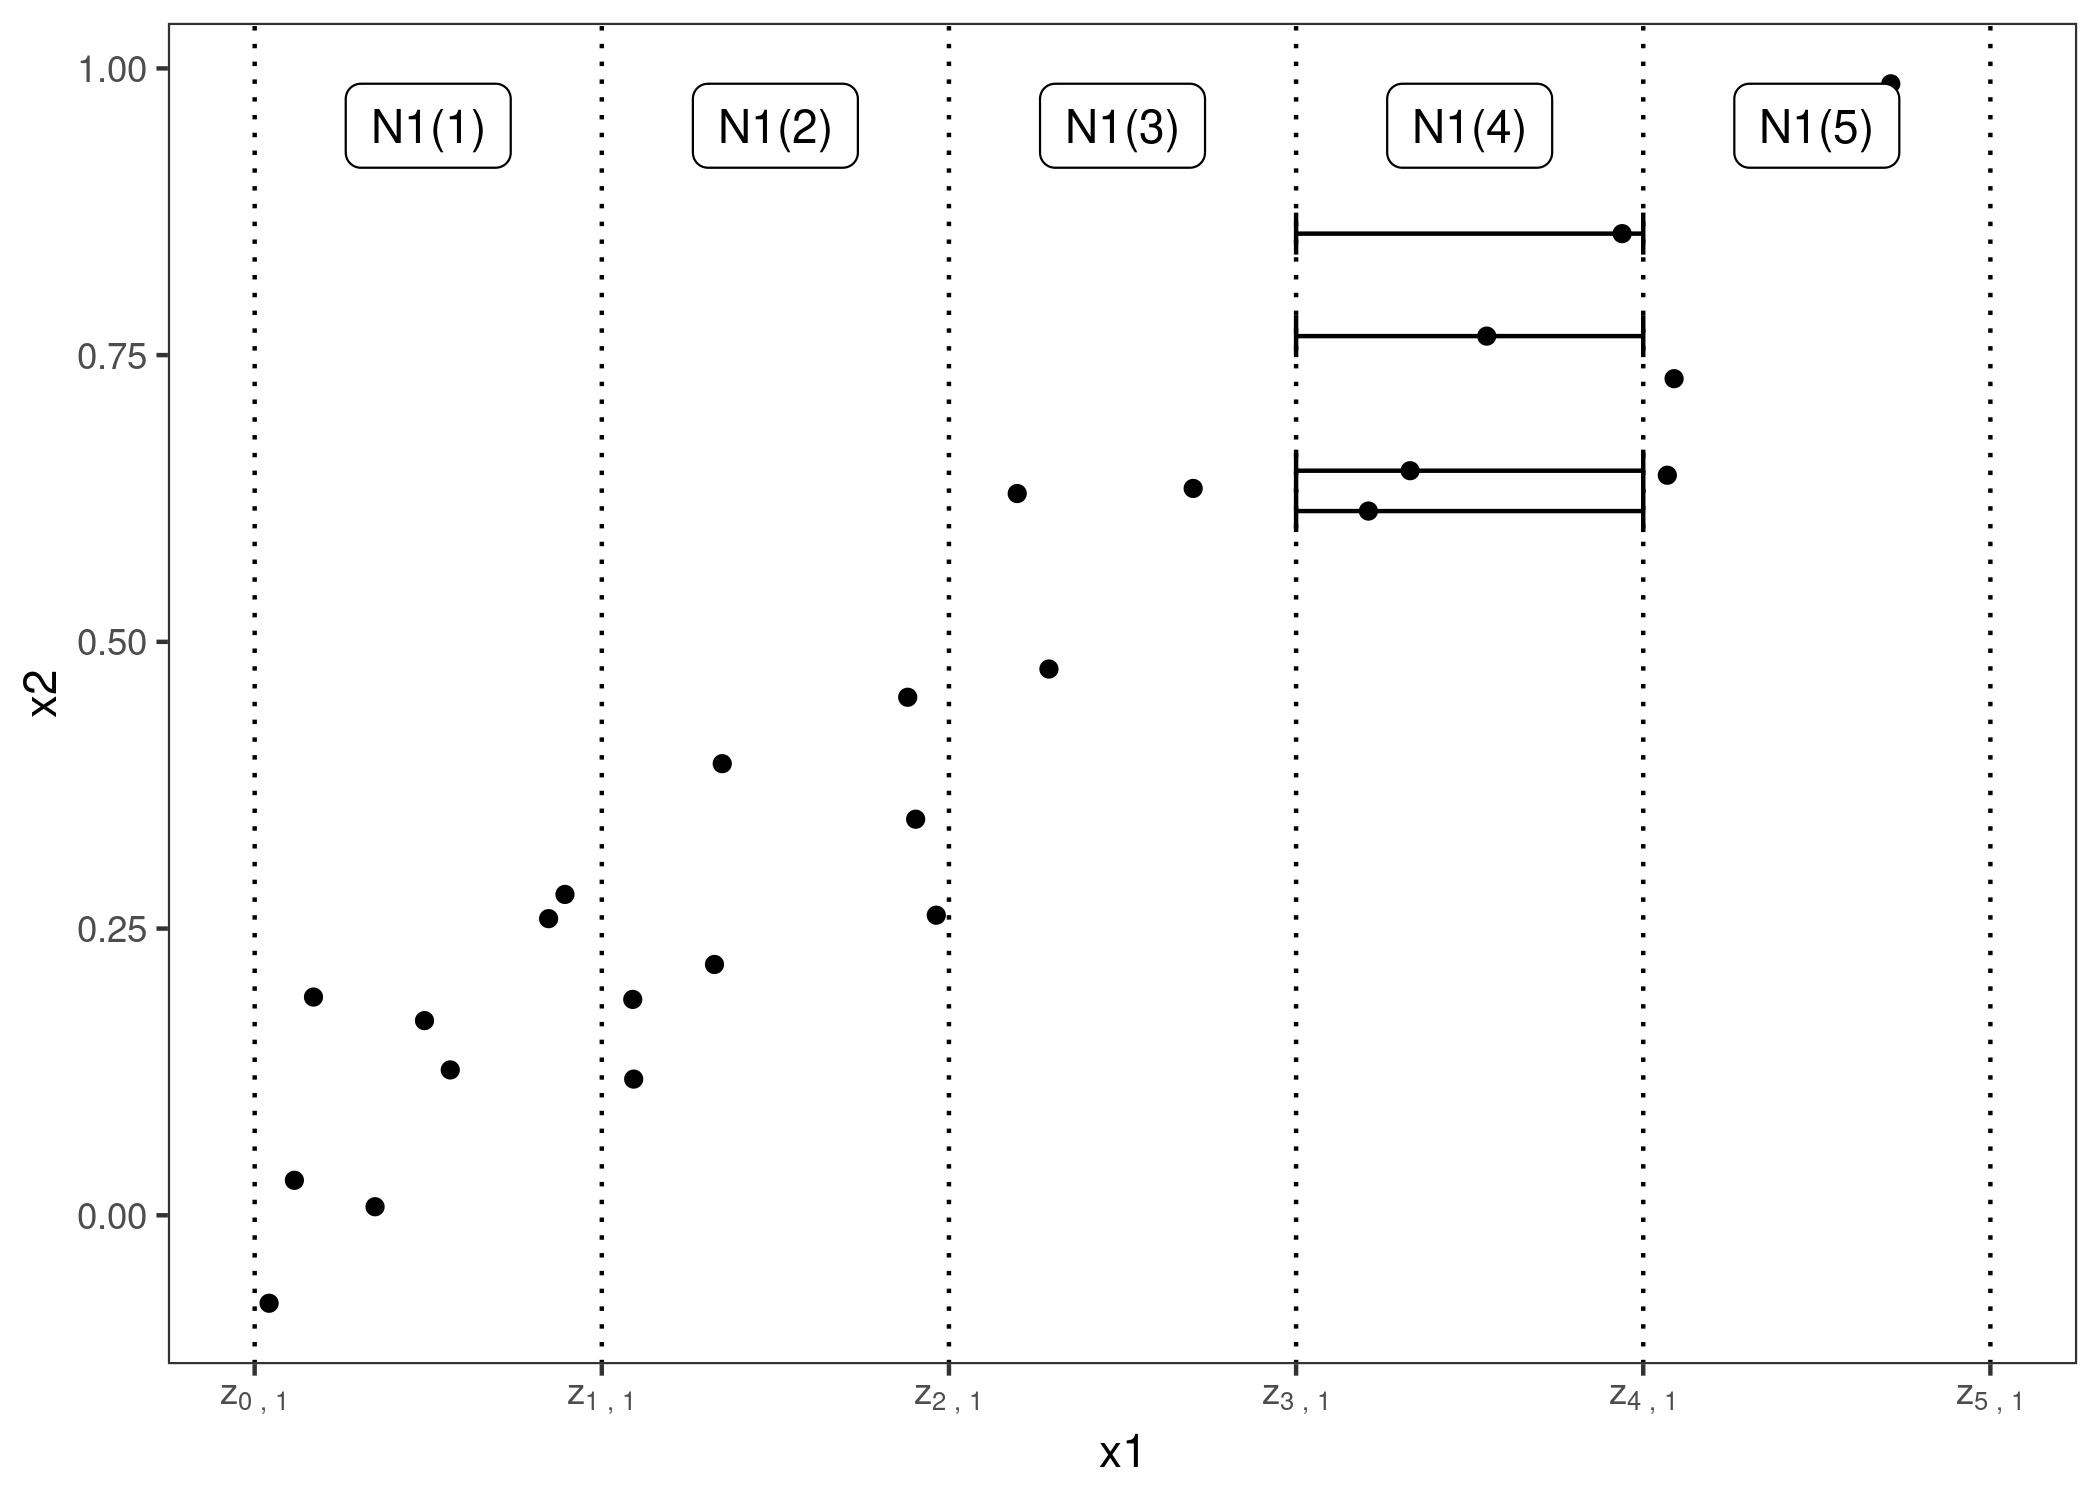
\includegraphics[height=3in]{molnar-8-7.jpeg} \\

\scriptsize Source: Molnar, Fig. 8.7
\end{frame}

\begin{frame}[fragile]{Accumulated Local Effects (ALE) Plot}
Train model:
\begin{pythoncode}
from sklearn.tree import DecisionTreeRegressor
regr=DecisionTreeRegressor(min_samples_leaf=10).fit(x,y)
\end{pythoncode}
Construct the ALE and plot:
\begin{pythoncode}
import matplotlib.pyplot as plt
from PyALE import ale
ale_effects = ale(X=x, model=regr, \
    feature=['temp'], grid_size=50, include_CI=True)
plt.show()
\end{pythoncode}
2D feature interactions:
\begin{pythoncode}
ale_effects = ale(X=x, model=regr, \
    feature=['temp', 'hum'], grid_size=50)
plt.show()
\end{pythoncode}
\end{frame}

\begin{frame}{Accumulated Local Effects (ALE) Plot}
\centering 

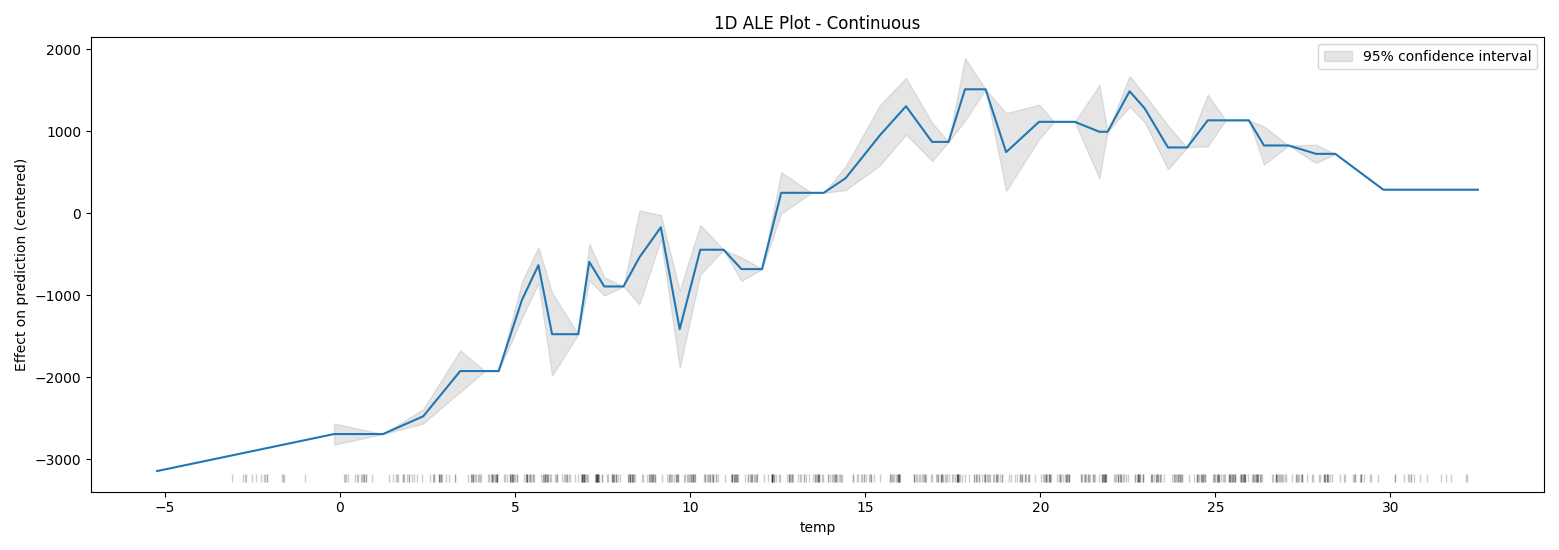
\includegraphics[height=1.5in]{ale_dtr.png} 

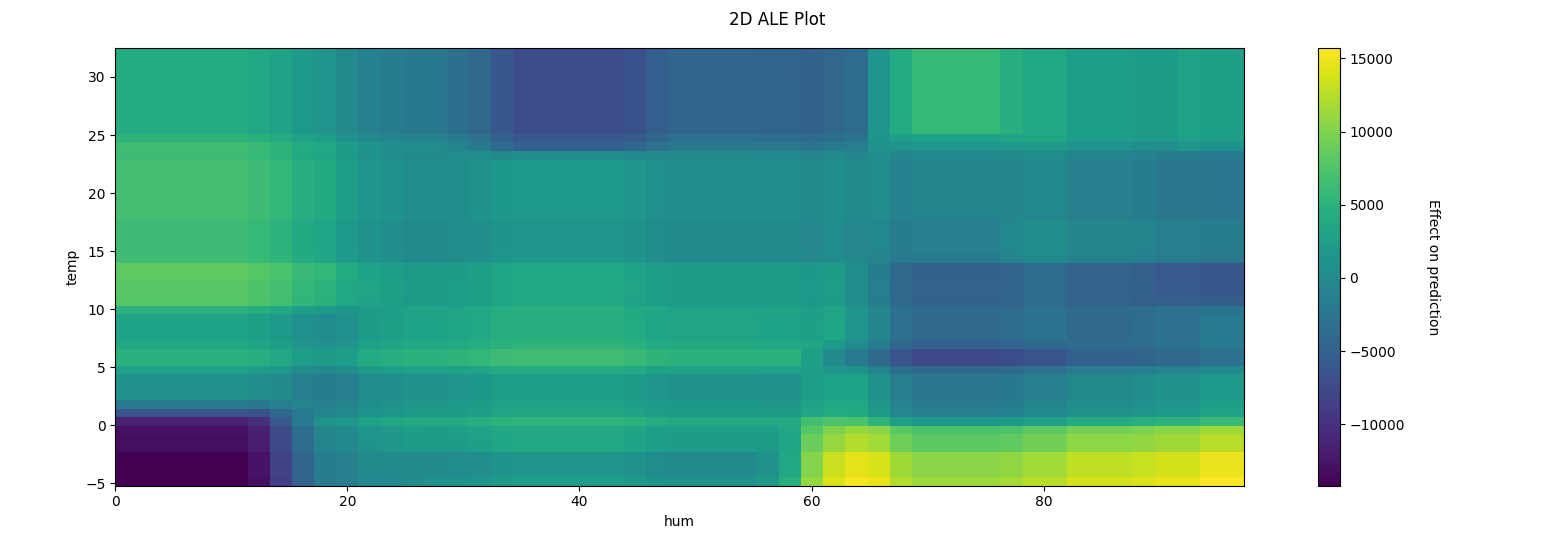
\includegraphics[height=1.5in]{2d_ale_dtr.png}

\end{frame}


\begin{frame}{Permutation Feature Importance}

\begin{block}{Intuition}
Calculate the increase in a model's prediction error when permuting a feature
\end{block}

\begin{enumerate}
\item Estimate model error on original data $e^{\text{orig}} = L(y, \hat{f}(X))$
\item For each feature $j$:
  \begin{itemize}
     \item For each repetition $k$ in $1 \cdots K$:
     \begin{itemize}
        \item Generate $X^{\text{perm}}_{j, k}$ by permuting (''randomly shuffling'') values of feature $j$
        \item Estimate $e^{\text{perm}}_{j, k} = L(y, \hat{f}(X^{\text{perm}}_{j, k}))$
     \end{itemize}
     \item Calculate permutation feature importance as $i_j = e^{\text{orig}} - \frac{1}{K}\sum_k^K e^{\text{perm}}_{j, k}$
  \end{itemize}
\end{enumerate}
\begin{block}{}
Calculate Permutation Feature Importance on \emph{test} data
\end{block}
\end{frame}

\begin{frame}[fragile]{Permutation Feature Importance}
Prepare data:
\begin{pythoncode}
import pandas as pd
d=pd.read_csv('https://evermann.ca/busi4720/bike.csv')
x=pd.get_dummies(d.drop(['yr','days_since_2011'],axis=1))
y=x.pop('cnt')
\end{pythoncode}
Train model:
\begin{pythoncode}
from sklearn.tree import DecisionTreeRegressor
regr=DecisionTreeRegressor(min_samples_leaf=10).fit(x,y)
\end{pythoncode}
Calculate permutation feature importance and sort them:
\begin{pythoncode}
from sklearn.inspection import permutation_importance
r = permutation_importance(regr, x, y, n_repeats=30)
r_idx = r.importances_mean.argsort()
\end{pythoncode}
\end{frame}

\begin{frame}[fragile]{Permutation Feature Importance}
Produce a nice plot of sorted feature importance:
\begin{pythoncode}
import matplotlib.pyplot as plt
fig, ax = plt.subplots()
ax.boxplot(
    r.importances[r_idx].T,
    vert=False,
    labels=x.columns[r_idx])
ax.axvline(x=0, color="k", linestyle="--")
plt.show()
\end{pythoncode}
\end{frame}

\begin{frame}{Permutation Feature Importance}
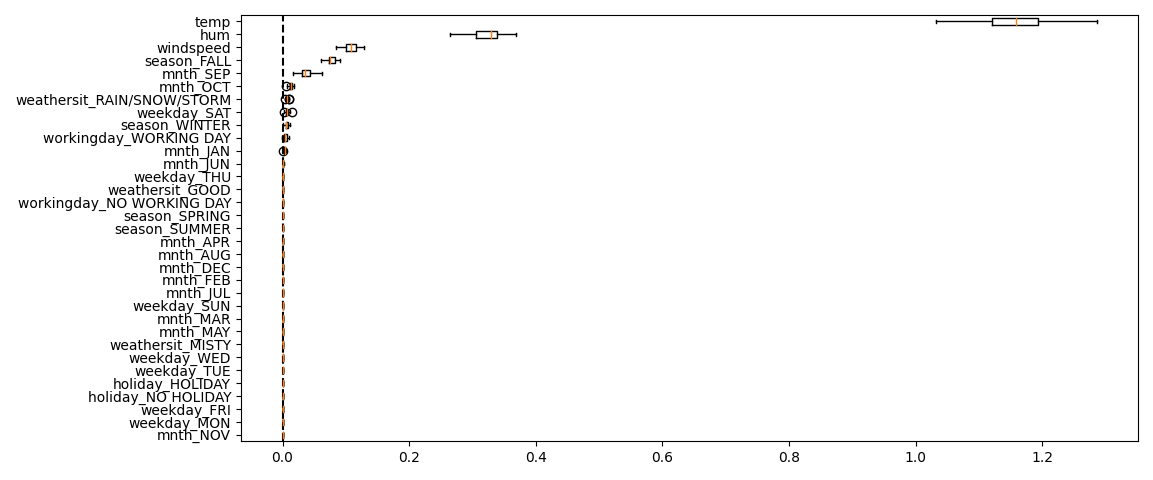
\includegraphics[width=\textwidth]{pfi_tree.png} \\

\footnotesize Uncertainty due to multiple permutations (parameter \texttt{n\_repeats})
\end{frame}

\begin{frame}[fragile]{Global Surrogate Models}
\begin{block}{Intuition}
Predict the predictions of a complex ''black box'' model using an intrinsically interpretable model.
\end{block}
Example ''black box'' model:
\begin{pythoncode}
from sklearn.neural_network import MLPRegressor
regr = MLPRegressor((4, 2,), max_iter=10000)
regr.fit(x, y)
preds = regr.predict(x)
\end{pythoncode}
Interpretable, linear model to explain predictions:
\begin{pythoncode}
from statsmodels.api import OLS
OLS(preds, x).fit().summary()
\end{pythoncode}
\end{frame}

\begin{frame}{Global Model Agnostic Methods -- Summary}
\footnotesize
\renewcommand{\arraystretch}{1.1}
\begin{tabular}{l|l} \hline
\multicolumn{2}{c}{\textbf{PDP/ICE}} \\ \hline
Intuitive & Limited number of features \\
Clear interpretation & Assumes feature independence \\
Easy to implement & \\ \hline
\multicolumn{2}{c}{\textbf{ALE}} \\ \hline
Unbiased for correlated features & Local interpretation only\\
Clear interpretation & ALE may differ from linear coefficients\\ 
Faster to compute than PDP & No ICE curves \\
& Unstable for large number of intervals \\  \hline
\multicolumn{2}{c}{\textbf{PFI}} \\ \hline
Clear interpretation & Linked to model error \\
Concise, global measure & Requires access to true targets \\
Does not require retraining & May be biased for correlated features \\
Takes into account all interactions & \\ \hline
\multicolumn{2}{c}{\textbf{Global Surrogate Models}} \\ \hline
Flexible & Conclusions about model, not data \\ 
Intuitive & Unclear cut-off for goodness of fit \\
R-squared measure for fit & \\ \hline
\end{tabular}
\end{frame}

\begin{frame}{Local Interpretable Model-Agnostic Explanations}
\small
\begin{block}{Idea}
\begin{enumerate}
   \item Choose an instance $x$ of interest, 
   \item Sample instances around it, weight by distance kernel $\pi_g$,
   \item Construct local interpretable model $g$
   \begin{itemize}
   \item Minimize discrepancy $\mathcal{L}$ between $g$ and black-box model $f$
   \item Penalize by model complexity $\Omega(g)$
   \end{itemize}
\begin{align*}
\xi(x) = \operatorname*{argmin}_{g \in G} \; \mathcal{L} (f, g, \pi_x) + \Omega(g)
\end{align*}
\end{enumerate}
\end{block}


\begin{block}{Method}
\begin{enumerate}
  \item Sample instances $z'_i$ around $x'$ (interpretable version of $x$)
  \item Traing interpretable model on features $z'_i$, targets $f(z_i)$ and weights $\pi_x(z_i)$ ($z_i$ is the original version of $z'_i$)
\end{enumerate}
\end{block}
\end{frame}

\begin{frame}{LIME -- Example}
\begin{columns}
\begin{column}{.8\textwidth}
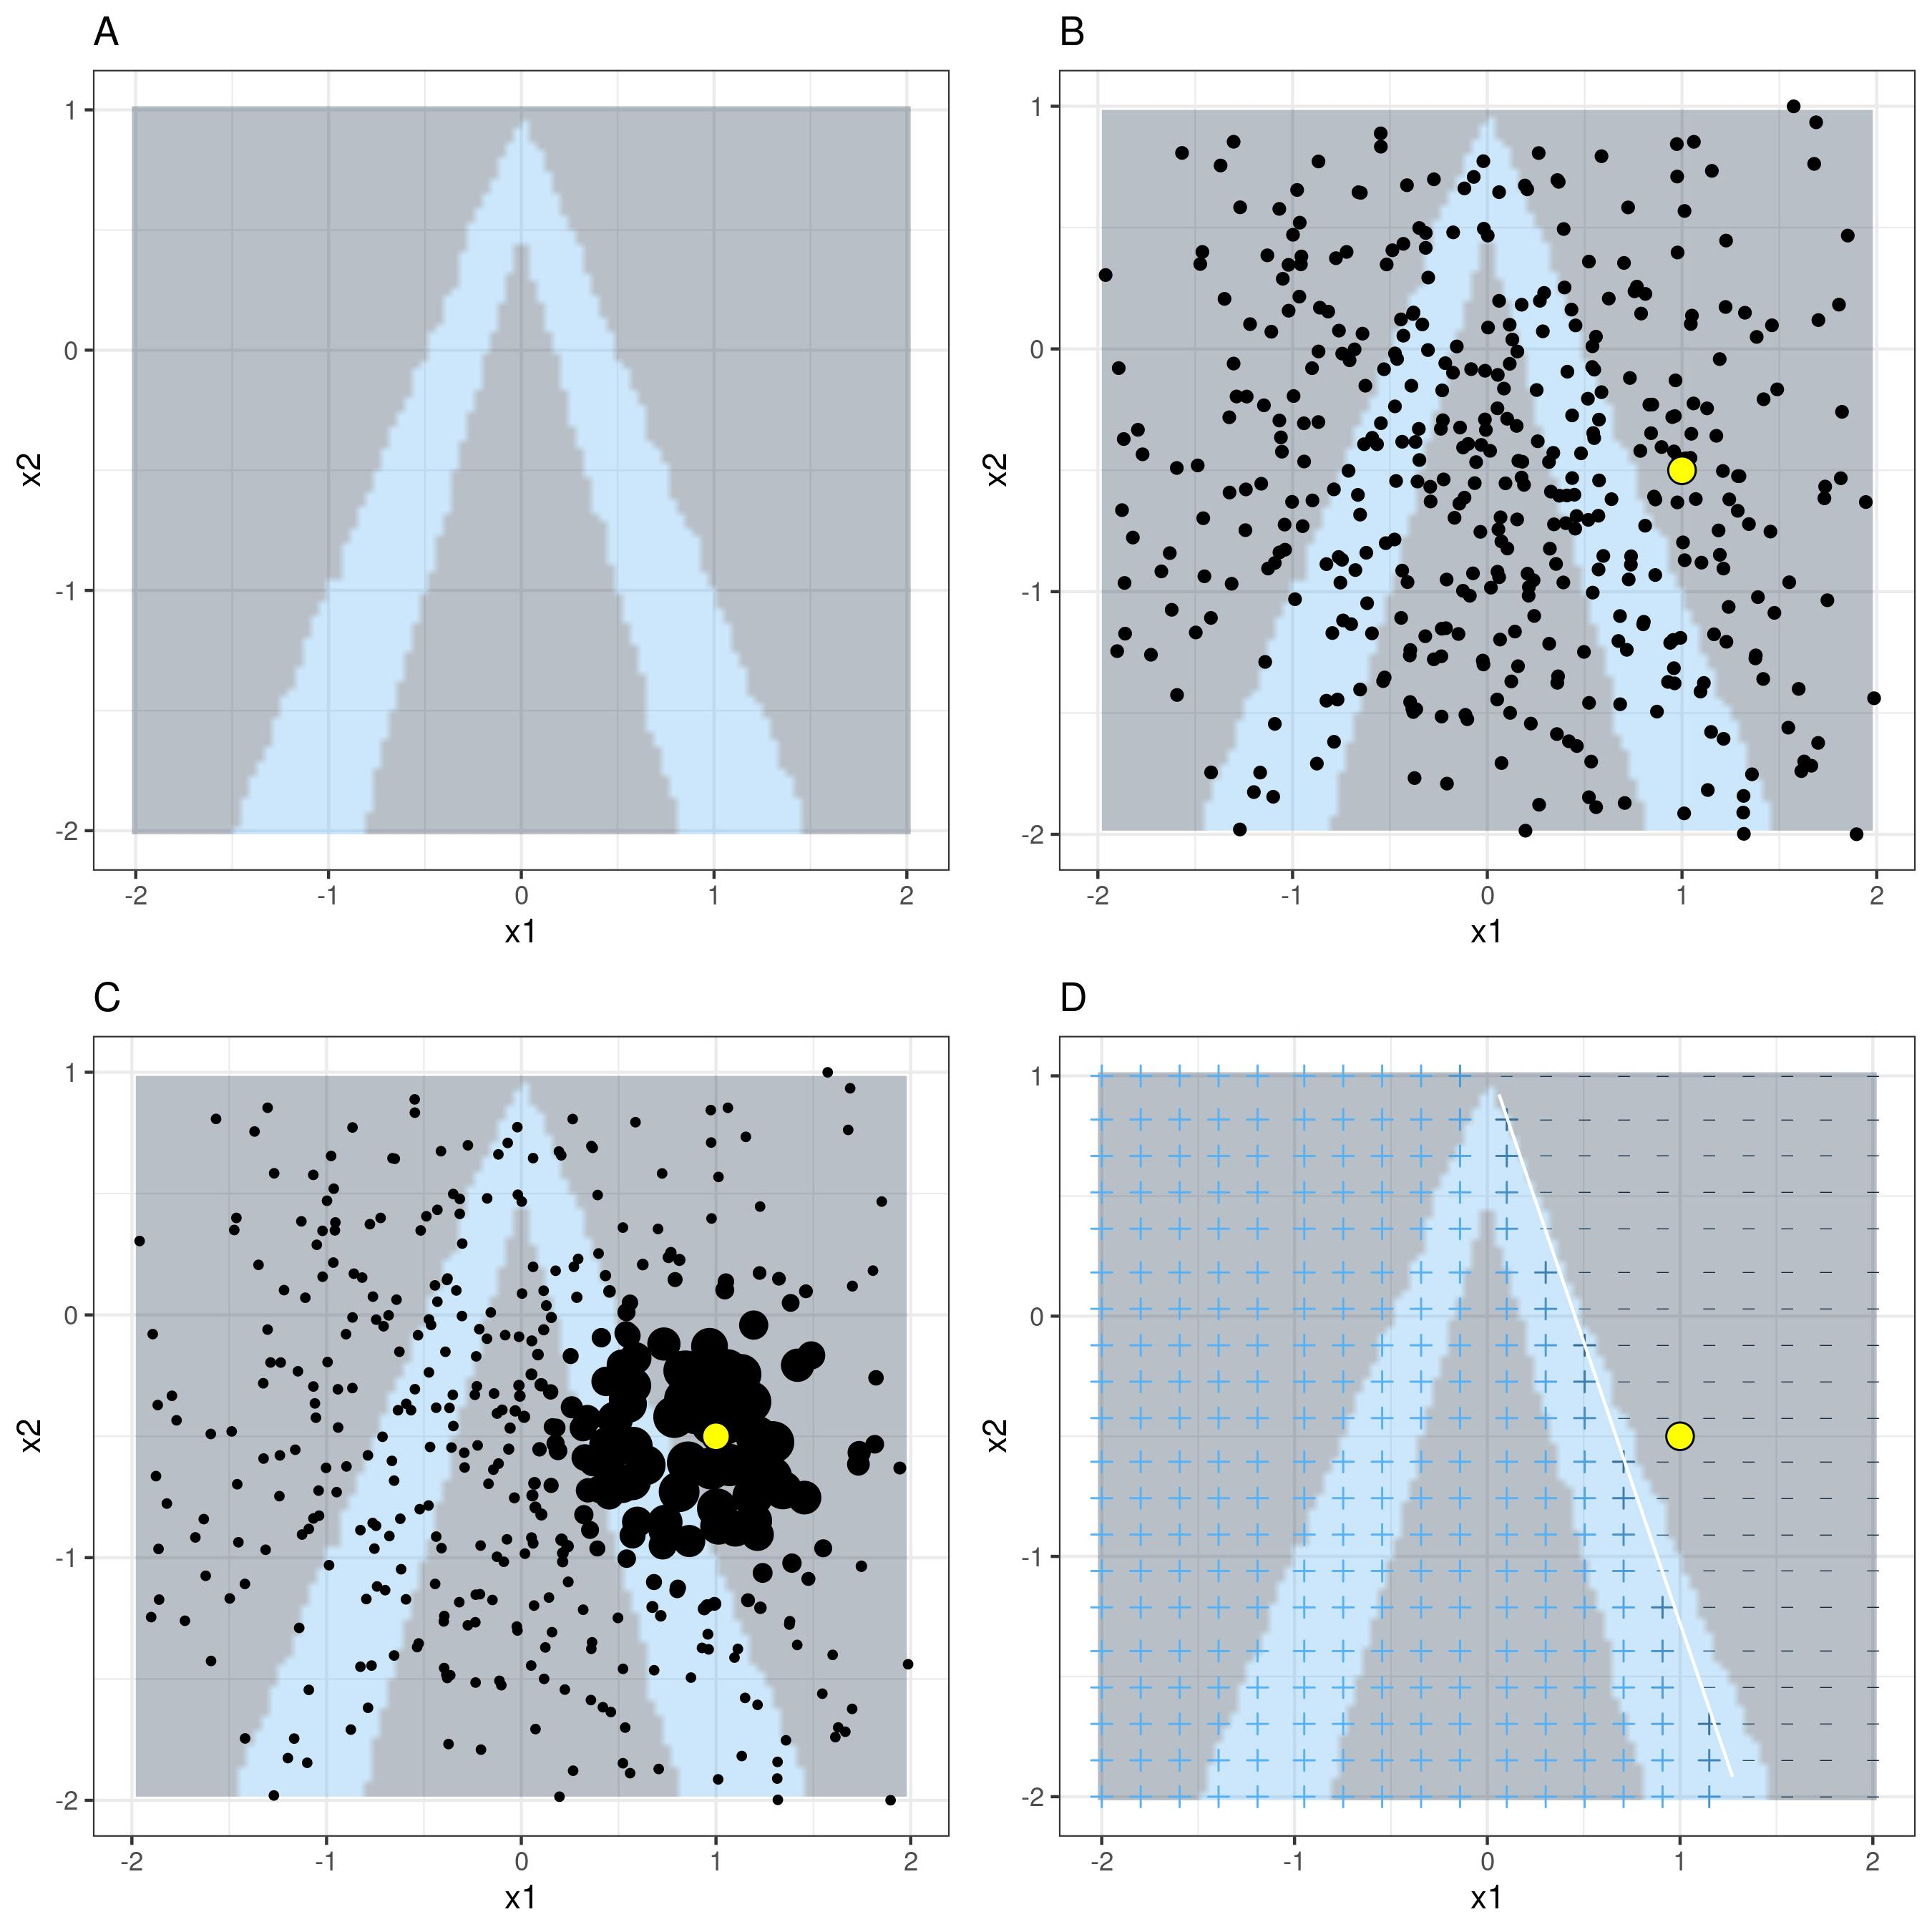
\includegraphics[height=3.25in]{molnar-9-5.jpeg} 
\end{column}
\begin{column}{.2\textwidth}
\scriptsize Source: Molnar Figure 9.5
\end{column}
\end{columns}
\end{frame}

\begin{frame}{LIME -- Example}
\begin{itemize}
   \item Weight function $\pi$ is often an exponential smoothing kernel
   \item Kernel width is critical determinant of explanation
\end{itemize}
\begin{columns}
\begin{column}{.9\textwidth}
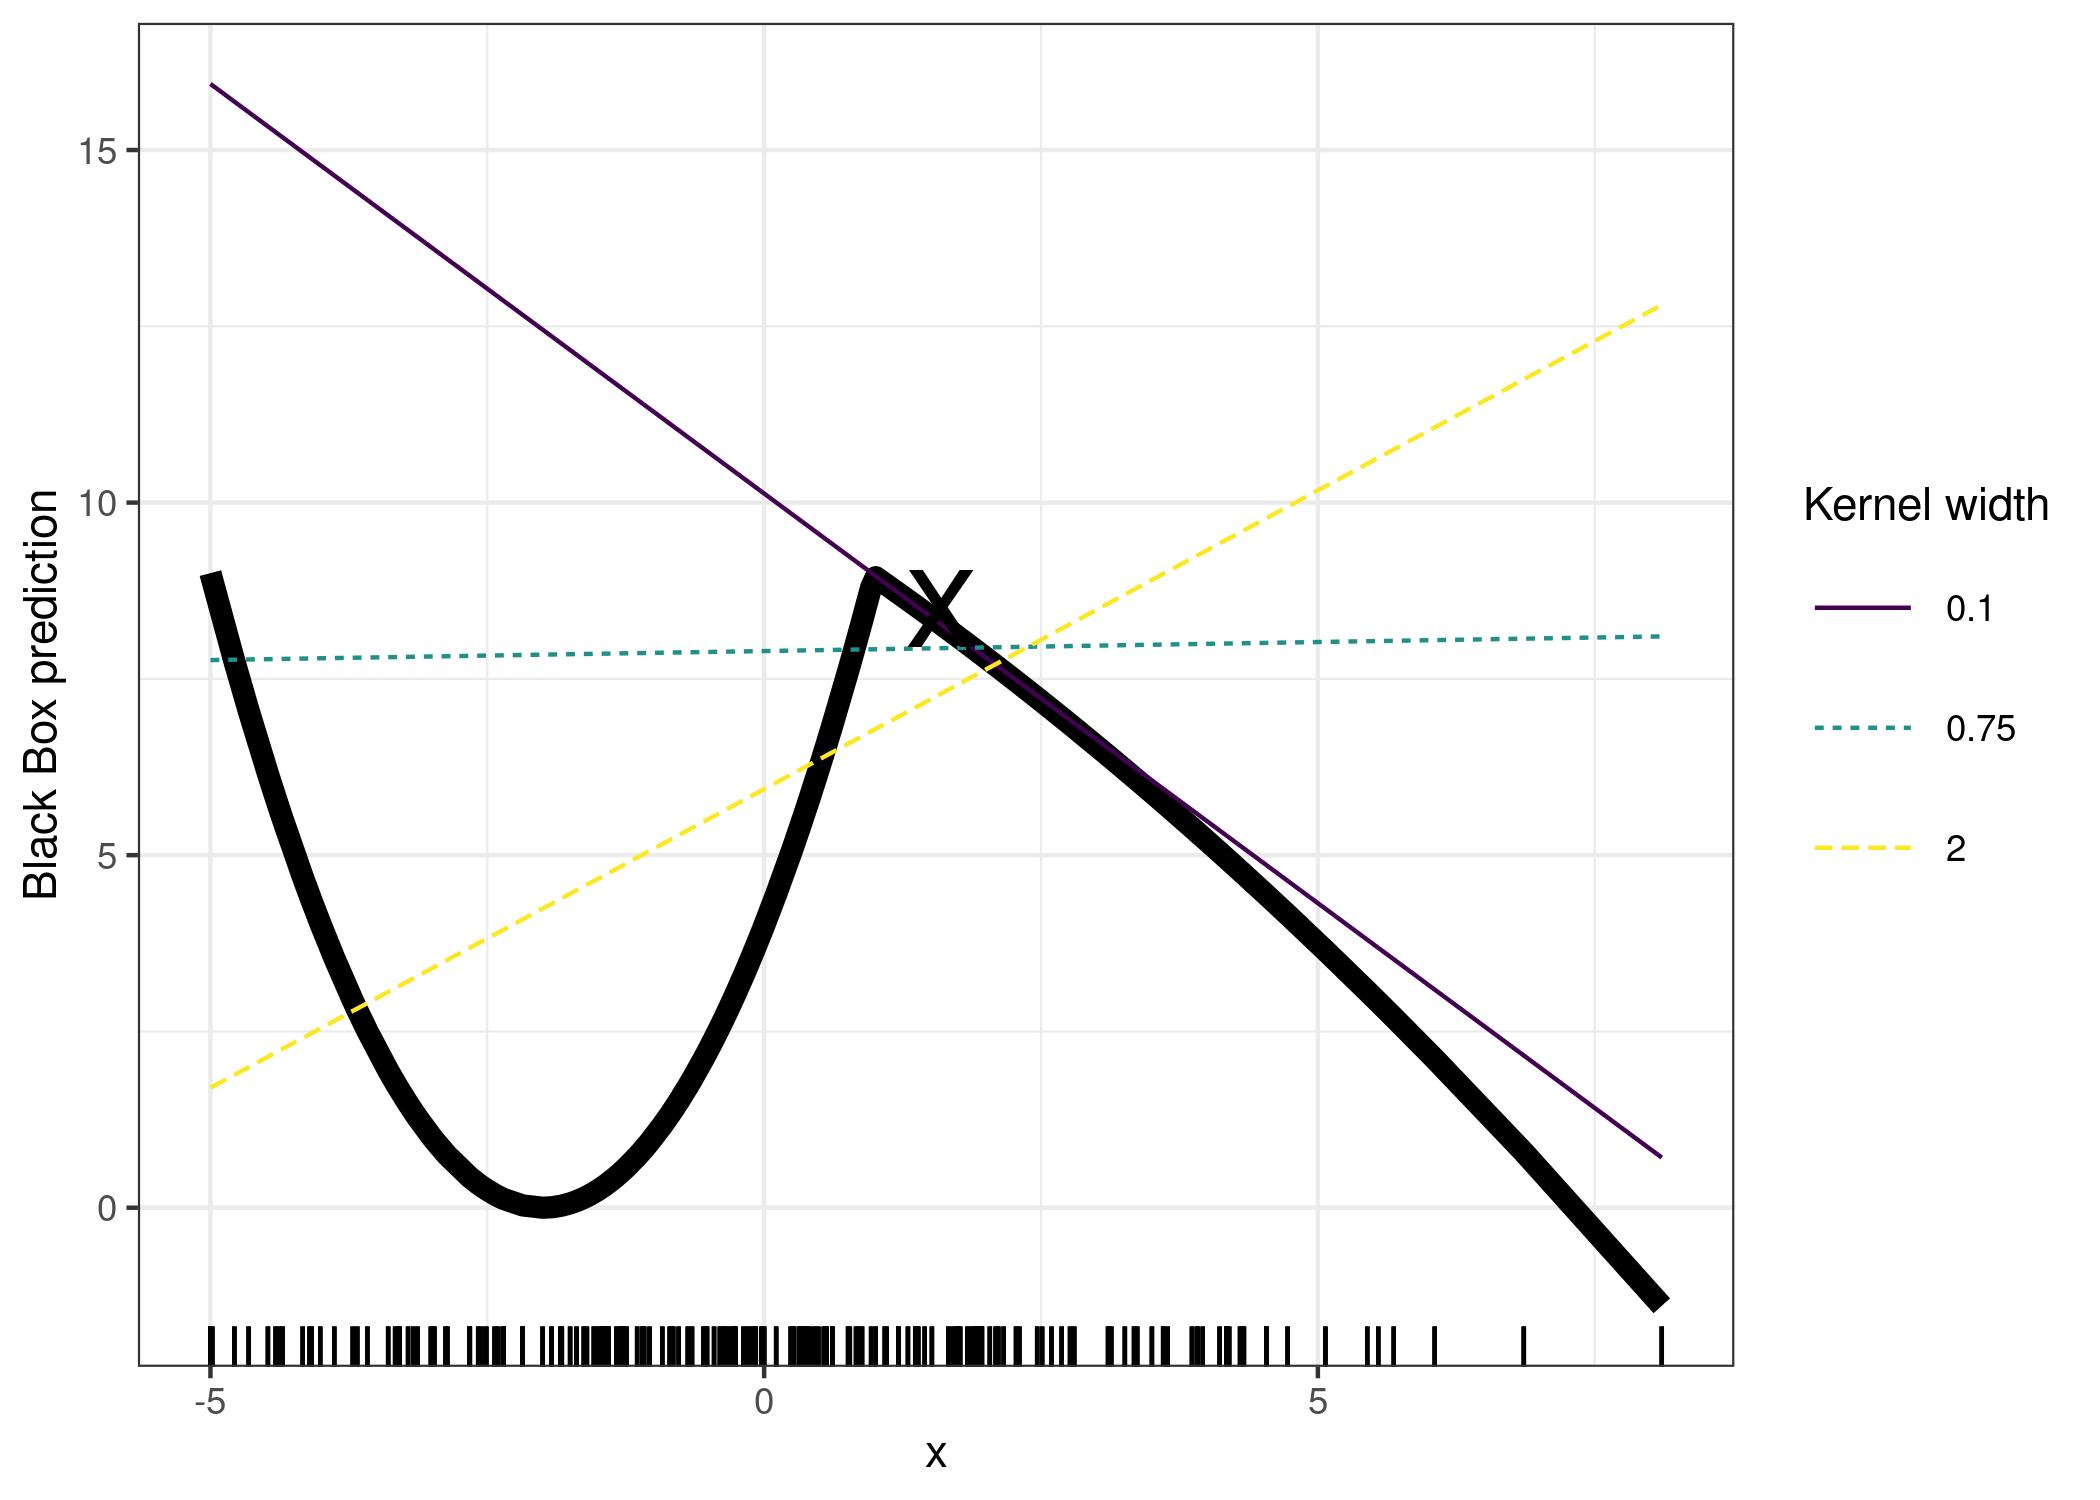
\includegraphics[height=2.75in]{molnar-9-6.jpeg}
\end{column}
\begin{column}{.15\textwidth}
\scriptsize Source: Molnar Figure 9.6
\end{column}
\end{columns}
\end{frame}

\begin{frame}[fragile]{LIME -- Example}
Using a deep decision tree as ''black box'':
\begin{pythoncode}
import sklearn.tree
dt = sklearn.tree.DecisionTreeClassifier(max_depth=8)
dt.fit(x, y)
\end{pythoncode}
Create the explainer:
\begin{pythoncode}
import lime, lime.lime_tabular
from sklearn.linear_model import Ridge

explainer = lime.lime_tabular.LimeTabularExplainer(
    x.to_numpy(), 
    feature_names=x.columns, 
    discretize_continuous = True, 
    mode='regression', 
    verbose=True)
\end{pythoncode}
\end{frame}

\begin{frame}[fragile]{LIME -- Example}
Explain instance number 5:
\begin{pythoncode}
exp = explainer.explain_instance( 
    x.to_numpy()[7], 
    dt.predict, 
    num_features=5, 
    num_samples=1000, 
    distance_metric='euclidean')
exp.as_list()
exp.as_pyplot_figure().show()
\end{pythoncode}
%\end{frame}

%\begin{frame}{LIME -- Example}
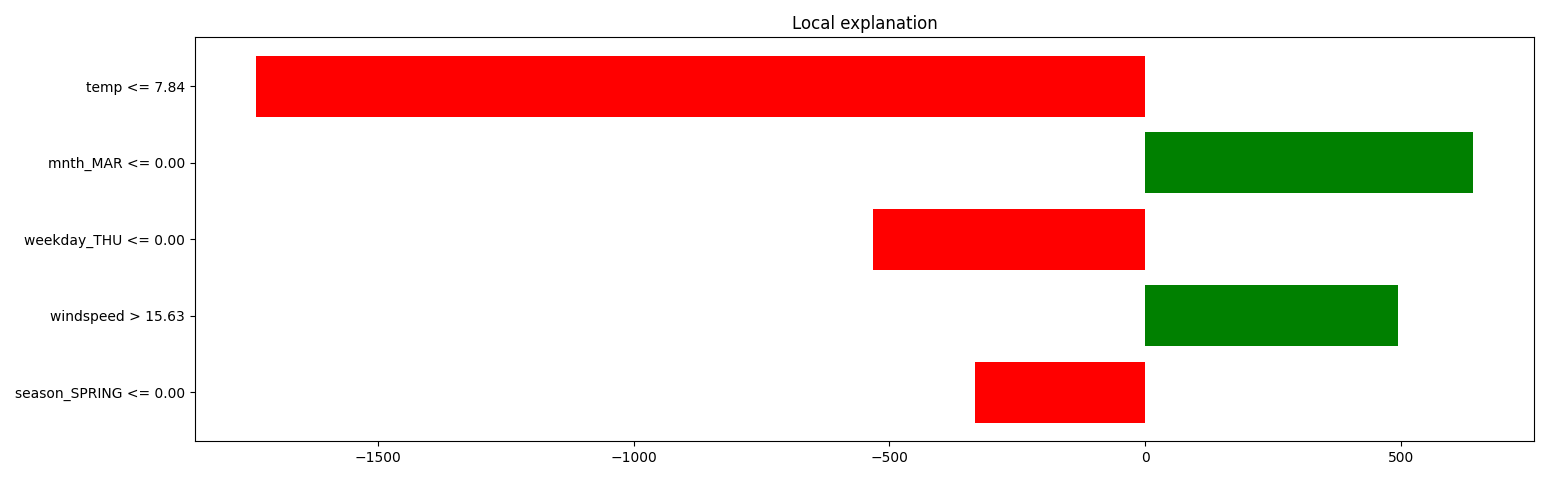
\includegraphics[width=\textwidth]{lime_dt.png}
\end{frame}

%\begin{frame}[fragile]{LIME -- Example}
%Key defaults in Python LIME:
%\begin{pythoncode}
%if kernel_width is None:
    %kernel_width=np.sqrt(training_data.shape[1])*.75

%if kernel is None:
    %def kernel(d, kernel_width):
        %return np.sqrt(np.exp(-(d**2)/kernel_width**2))
        
%if model_regressor is None:
    %model_regressor = Ridge(alpha=1,fit_intercept=True)
%\end{pythoncode}
%\end{frame}

\begin{frame}{LIME for Images}
LIME explanations for label ''bagel'' and ''strawberries'':
\begin{center}
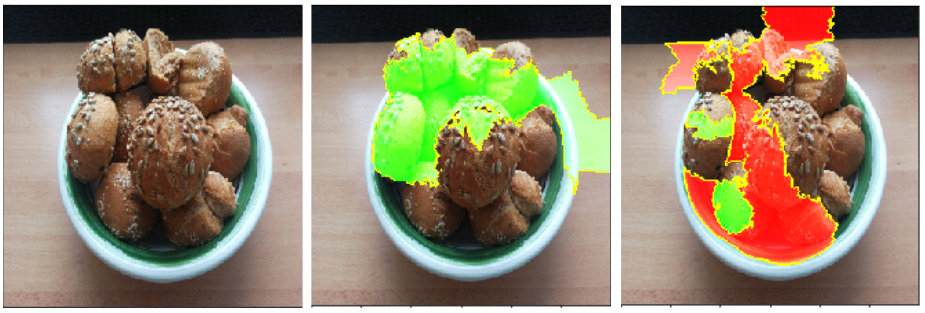
\includegraphics[width=\textwidth]{molnar-9-8.png} \\

\scriptsize Molnar, Figure 9.8
\end{center}
\begin{block}{Python Examples:}
\url{https://github.com/marcotcr/lime}
\end{block}

\begin{block}{Paper:}
\url{https://arxiv.org/abs/1602.04938}
\end{block}
\end{frame}


\begin{frame}{Shapley Values}
\begin{block}{Motivation}
How much does \emph{feature value} $x_j$ contribute to the overall prediction compared to the average prediction?
\end{block}

\begin{block}{Game Theory}
\begin{itemize}
\item Players cooperate in a coalition and receive a certain profit from this cooperation.
\item Method for assigning payouts to players depending on their contribution to the total payout. 
\end{itemize}
\end{block}

\end{frame}

\begin{frame}{Shapley Values}
\begin{align*}
\phi_i(v) = \frac{1}{n} \sum_{S \subseteq N \setminus \{i\}} \binom{n-1}{|S|}^{-1} \left[ v(S \cup \{i\}) - v(S)\right]
\end{align*}

\begin{itemize}
\item $v(S \cup \{i\}) - v(S)$: marginal contribution of player $i$ to coalition of players $S$
\item $\binom{n-1}{|S|}$: number of possible ways to form a coalition of size $|S|$ of the set $N \setminus \{i\}$ of $n-1$ players (set $N$ without player $i$)
\end{itemize}
\end{frame}

\begin{frame}{Shapley Value}
\begin{block}{Fairness Properties}
\begin{itemize}
   \item \textbf{Efficiency}: Contributions add up to total value
   \item \textbf{Symmetry}: If two players contribute equally to all possible coalitions, they have the same Shapley value
   \item \textbf{Dummy}: A player that does not contribute at all has a Shapley value of $0$
   \item \textbf{Additivity}: For a game with combined payouts $v + w$, the Shapley values of players are $\phi^{(v)} + \phi^{(w)}$
\end{itemize}
\end{block}
\end{frame}

\begin{frame}{Shapley Values in Interpretable ML}
\begin{itemize}
   \item Players are feature values
   \item Coalitions are combinations of feature values
   \item Presence in a coalition means we know the value
   \item Absence from a coalition means we don't know the value $\Rightarrow$ integrate/marginalize over all values of all features not in coalition $S$
   \begin{align*}
   v_x(S) = \idotsint_\Bbb{R} \hat{f}(x_1, \ldots, x_p) d\Bbb{P}_{x \not\in S} - E_x(\hat{f}(X))
   \end{align*}
   \item Expensive to compute $\Rightarrow$ in practice, approximation by sampling and permuting values (can make for unrealistic instances when features are correlated)
\end{itemize}
\end{frame}

\begin{frame}{Shapley Additive Explanations (SHAP)}
\small
\begin{columns}
\begin{column}{0.25\textwidth}
\centering


\includegraphics[width=.5\textwidth]{shap_logo.png} \\

\vspace{\baselineskip}
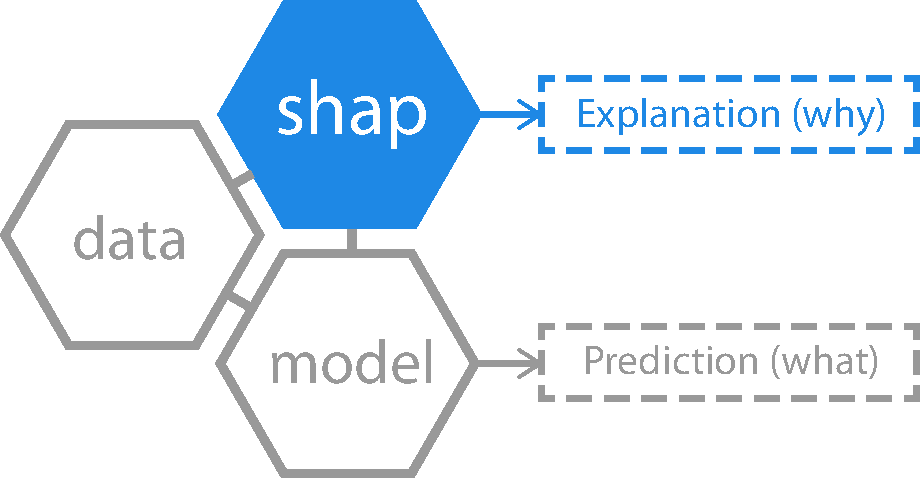
\includegraphics[width=\textwidth]{shap_logo.pdf}
\end{column}
\begin{column}{0.75\textwidth}
\begin{block}{Paper}
\url{https://arxiv.org/abs/1705.07874}
\end{block}

\begin{block}{Documentation (Intro and Examples)}
\url{https://shap.readthedocs.io/en/latest/index.html}
\end{block}

\begin{block}{Python Code and Tutorials}
\url{https://github.com/shap/shap}
\end{block}
\end{column}
\end{columns}

\end{frame}

%\begin{frame}{SHAP}
%\begin{itemize}
   %\item \textbf{Simplified inputs} $x'$ map to original inputs $x$ through a mapping function $x=h_x(x')$
   %\item \textbf{Local explanation methods} try to ensure that $g(z') \approx f(h_x(z'))$ whenever $z' \approx x'$
   %\item \textbf{Additive feature attribution methods} have an explanation model $g$ that is a linear function of binary variables:
   %\begin{align*}
   %g(z') = \phi_0 + \sum_{i=1}^M \phi_i z'_i
   %\end{align*}
   %where $z' \in \{0, 1\}^M$, $M$ is the number of simplified inputs and $\phi_i \in \Bbb{R}$ is the attributed effect
%\end{itemize}
%\end{frame}

%\begin{frame}{SHAP}
%\begin{block}{Properties}
%\begin{itemize}
   %\item \textbf{Local accuracy}: The explanation model $g(x')$ matches the original model $f(x)$ when $x = h_x(x')$
   %\item \textbf{Missingness}: Missingness constrains features where $x'_i=0$ to have no attributed effect
   %\item \textbf{Consistency}: If a model changes so that some simplified input's contribution increases or stays the same, that input's attributed effect should not decrease
%\end{itemize}
%\end{block}
%\centering

%Shapley values are the only additive feature attribution method satisfying these properties.
%\end{frame}

%\begin{frame}{SHAP}
%\textbf{Shapley kernel}: Shapley values can be recovered by LIME under the following assumptions:
%\begin{align*}
%\Omega(g) &= 0 \\
%\pi_{x'}(z') &= \frac{(M-1)}{\binom{M}{|z'|} |z'| (M - |z'|)} \\
%L(f, g, \pi_{x'}) &= \sum_{z' \in Z} \left[ f(h_x^{-1}(z')) - g(z') \right]^2 \phi_{x'}(z')
%\end{align*}
%\end{frame}

\begin{frame}[fragile]{SHAP Example}
Fit a simple regression model to the California housing dataset:
\begin{pythoncode}
import sklearn
import shap

X, y = shap.datasets.california(n_points=1000)
model = sklearn.linear_model.LinearRegression()
model.fit(X, y)
\end{pythoncode}
Compute the SHAP values:
\begin{pythoncode}
X100 = shap.utils.sample(X, 100)
explainer = shap.Explainer(model.predict, X100)
shap_values = explainer(X)
\end{pythoncode}
\end{frame}

\begin{frame}[fragile]{SHAP Example}
The \textbf{barplot} shows the importance of feature values for an individual prediction:
\begin{pythoncode}
shap.plots.bar(shap_values[20])
\end{pythoncode}
\begin{center}
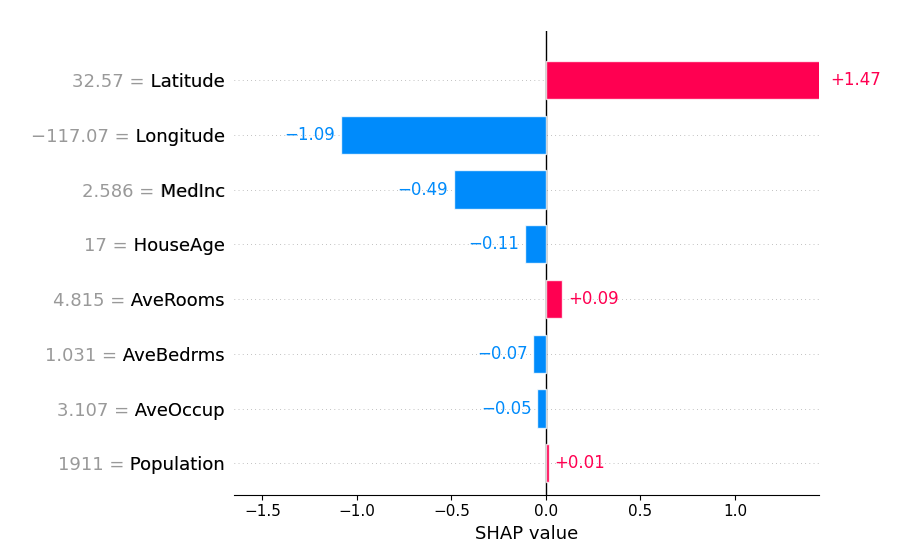
\includegraphics[height=2in]{shap_barplot1.png}
\end{center}
\end{frame}

\begin{frame}[fragile]{SHAP Example}
The \textbf{barplot} can also show the importance of a feature by averaging over all instances (and their feature values):
\begin{pythoncode}
shap.plots.bar(shap_values)
\end{pythoncode}
\begin{center}
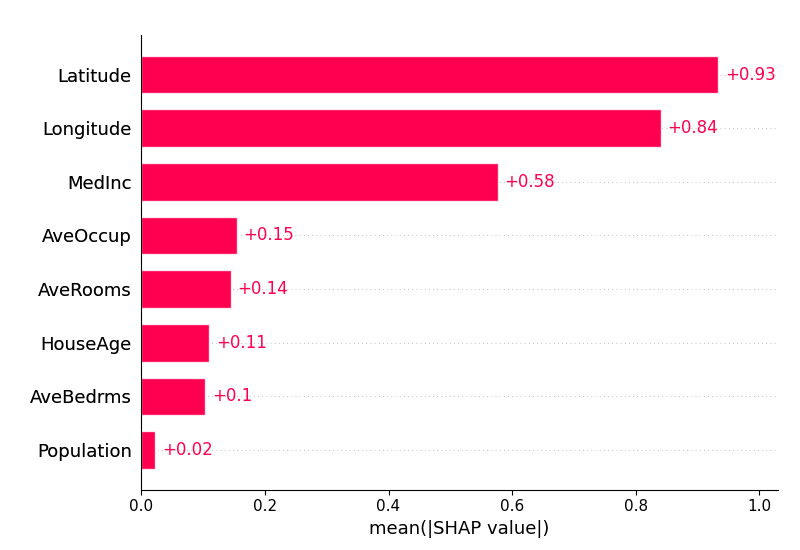
\includegraphics[height=2in]{shap_barplot2.png}
\end{center}
\end{frame}

\begin{frame}[fragile]{SHAP Example}
\textbf{Waterfall plots} explain how feature values combine to produce an individual prediction:
\begin{pythoncode}
sha.plots.waterfall(shap_values[20], max_display=14)
\end{pythoncode}
\begin{center}
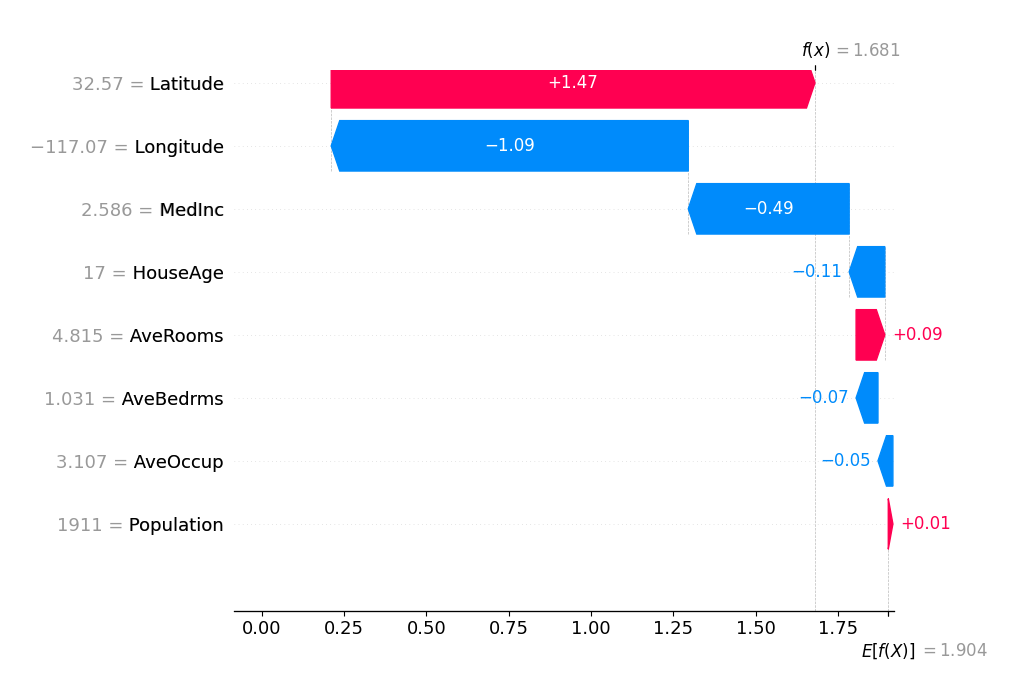
\includegraphics[height=2in]{shap_waterfall1.png}
\end{center}
\end{frame}

\begin{frame}[fragile]{SHAP Example}
\textbf{Beeswarm plots} explain all feature values for all instances (represented by a dot):
\begin{pythoncode}
shap.plots.beeswarm(shap_values)
\end{pythoncode}
\begin{center}
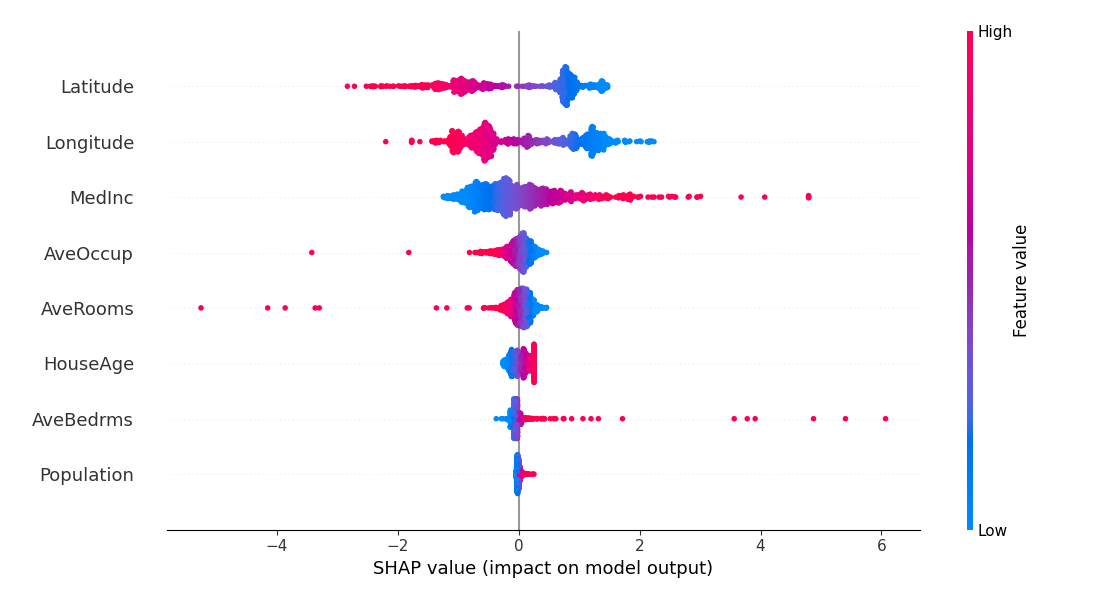
\includegraphics[height=2in]{shap_beeswarm1.png}
\end{center}
\end{frame}

\begin{frame}[fragile]{SHAP Example}
The \textbf{heatmap} shows SHAP values of feature values for all instances, and shows model prediction and global feature importance in rugs:
\begin{pythoncode}
shap.plots.heatmap(shap_values)
\end{pythoncode}
\begin{center}
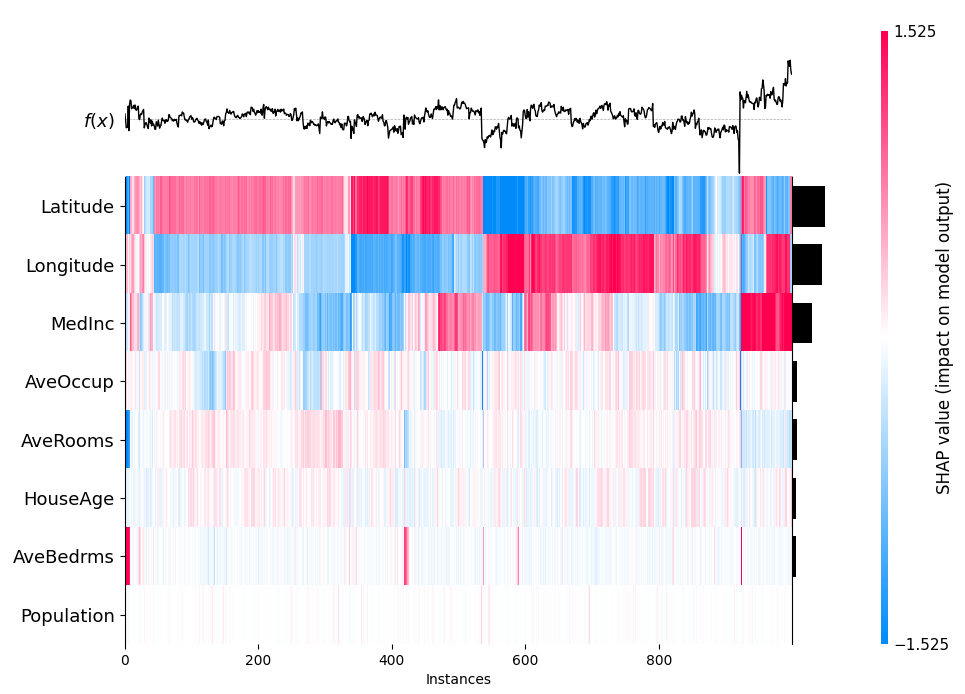
\includegraphics[height=2in]{shap_heatmap1.png}
\end{center}
\end{frame}

\begin{frame}{SHAP for Image Classification}
\begin{itemize}
\item Presence/absence of features/pixels by masking parts of an image:
\end{itemize}

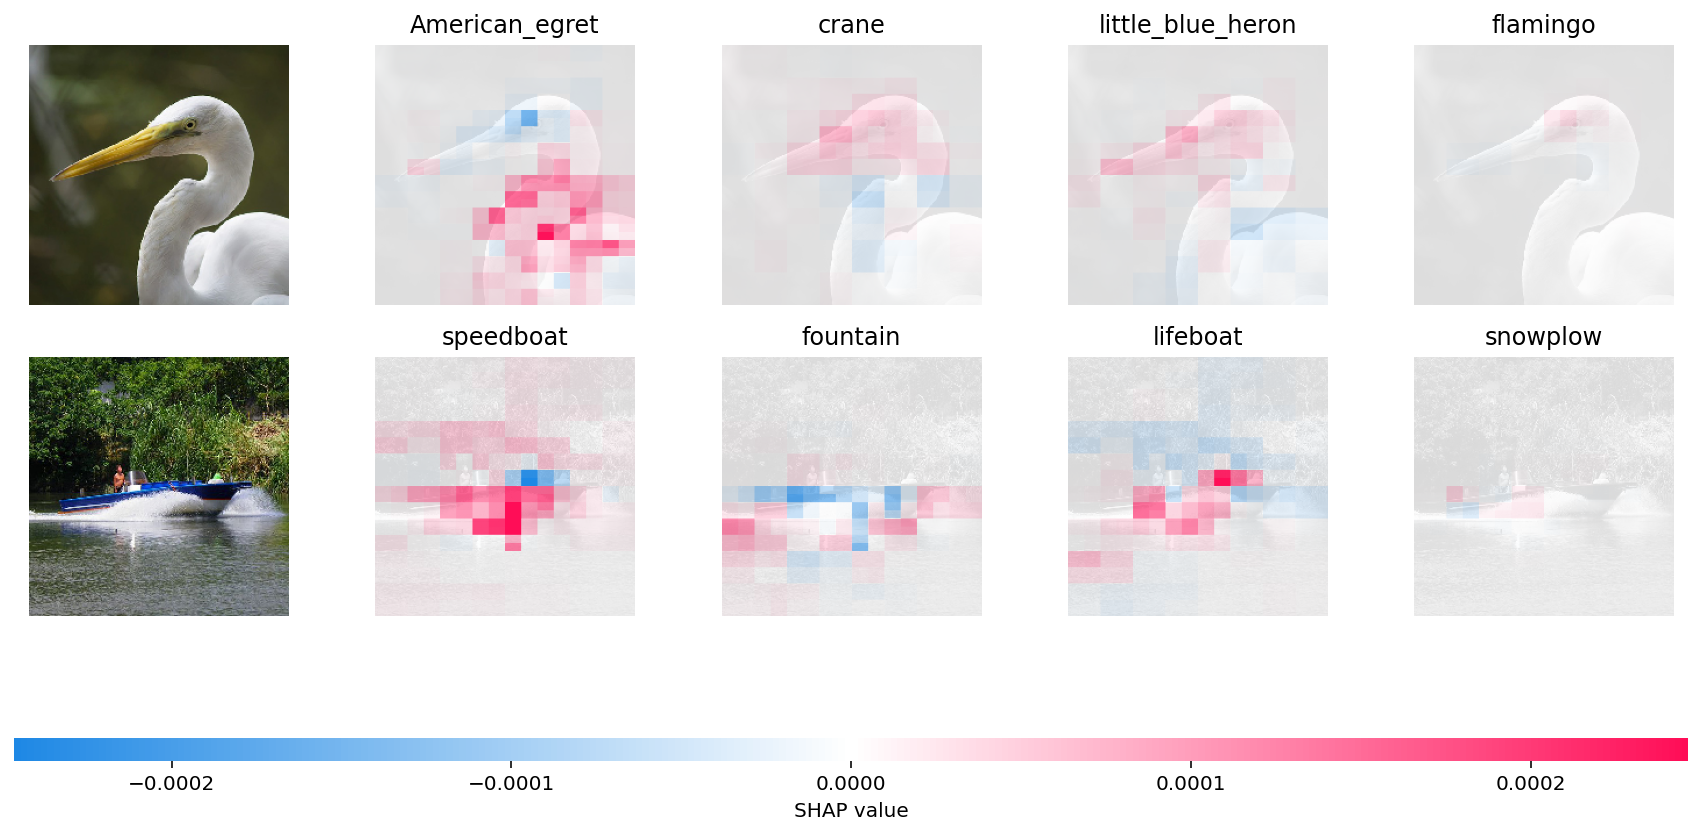
\includegraphics[width=\textwidth]{shap_image.png} \\

\scriptsize Source: \url{https://github.com/shap} (MIT License)
\end{frame}

\begin{frame}{SHAP for Text Classification}
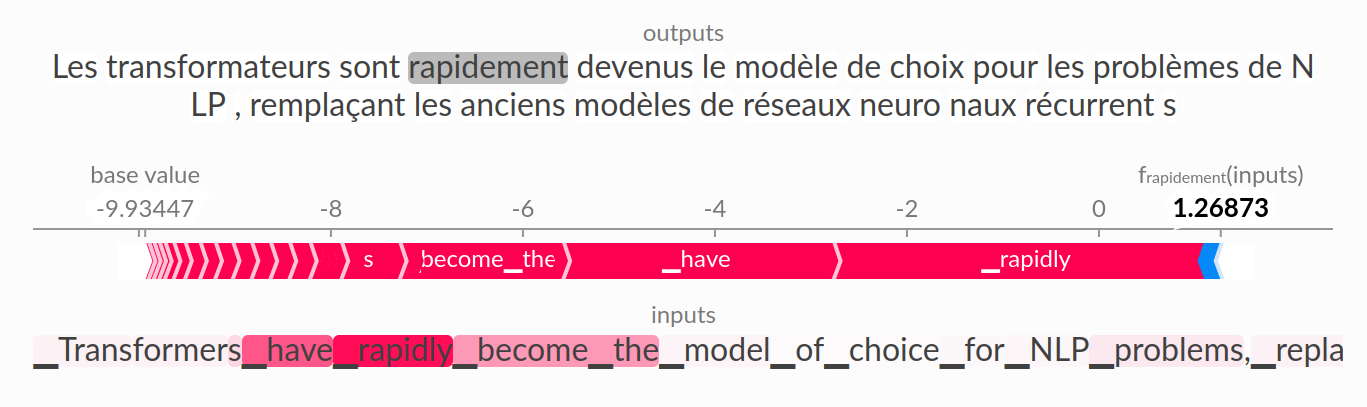
\includegraphics[width=\textwidth]{shap_text.png} \\

\scriptsize Source: \url{https://shap.readthedocs.io/en/latest/text_examples.html} (MIT License)
\end{frame}

\end{document}




